\chapter{On confident outrankings with uncertain criteria significance weights}
\label{sec:18}

\abstract*{ When modelling preferences following the outranking approach, the signs of the majority margins do sharply distribute validation and invalidation of pairwise outranking situations. How can we be confident in the resulting outranking digraph, when we acknowledge the usual imprecise knowledge of criteria significance weights coupled with small majority margins? In this chapter we propose to link the qualifying significance majority with a required $\alpha\%$-confidence level. We model therefore the significance weights as random variables following more or less widespread distributions around an average significance value that corresponds to the given deterministic weight. As the bipolar-valued random credibility of an outranking statement hence results from the simple sum of positive or negative independent random variables, we may apply the Central Limit Theorem (CLT) for computing the bipolar likelihood that the expected majority margin will indeed be positive, respectively negative.}

\abstract{ When modelling preferences following the outranking approach, the signs of the majority margins do sharply distribute validation and invalidation of pairwise outranking situations. How can we be confident in the resulting outranking digraph, when we acknowledge the usual imprecise knowledge of criteria significance weights coupled with small majority margins? In this chapter we propose to link the qualifying significance majority with a required $\alpha\%$-confidence level. We model therefore the significance weights as random variables following more or less widespread distributions around an average significance value that corresponds to the given deterministic weight. As the bipolar-valued random credibility of an outranking statement hence results from the simple sum of positive or negative independent random variables, we may apply the Central Limit Theorem (CLT) for computing the bipolar likelihood that the expected majority margin will indeed be positive, respectively negative.}

\section{Modelling uncertain criteria significance weights}
\label{sec:18.1}

Let us consider the significance weights of a family $F$ of $m$ criteria to be independent random variables $W_j$, distributing the potential significance weight of each criterion $j = 1, ..., m$ around a mean value $E(W_j)$ with variance $V(W_j)$.

Choosing a specific stochastic model of uncertainty is usually application specific. In the limited scope of this chapter, we will illustrate the consequence of this design decision on the resulting outranking modelling with four slightly different models for taking into account the uncertainty with which we know the numerical significance weights: \emph{uniform}, \emph{triangular}, and two models of \emph{Beta laws}, one more widespread and, the other, more concentrated.

When considering, for instance, that the potential range of a significance weight is distributed between $0$ and two times its mean value, we obtain the following random variates \citep{CPSTAT-L3}:
\begin{itemize}[topsep=2pt]
\item A continuous \emph{uniform} distribution on the range $0$ to $2E(W_j)$. Thus $W_j \leadsto U(0, 2E(W_j))$ and $V(W_j) = 1/3(E(W_j))^2$;
\item A \emph{symmetric beta} distribution with, for instance, parameters  $\alpha = 2$ and $\beta = 2$. Thus, $W_i \leadsto Beta(2,2) \times 2E(W_j)$ and $V(W_j) = 1/5(E(Wj))^2$;
\item A \emph{symmetric triangular} distribution on the same range wit mode $E(W_j)$. Thus $W_j \leadsto Tr(0, 2E(W_j), E(Wj))$ with $V(W_j) = 1/6(E(Wj))^2$;
\item A \emph{narrower beta} distribution with, for instance, parameters $\alpha = 4$ and $\beta = 4$. Thus $W_j \leadsto Beta(4,4) \times 2E(W_j)$ , $V(W_j) = 1/9(E(W_j))^2$.
\end{itemize}
\begin{figure}[ht]
%\sidecaption
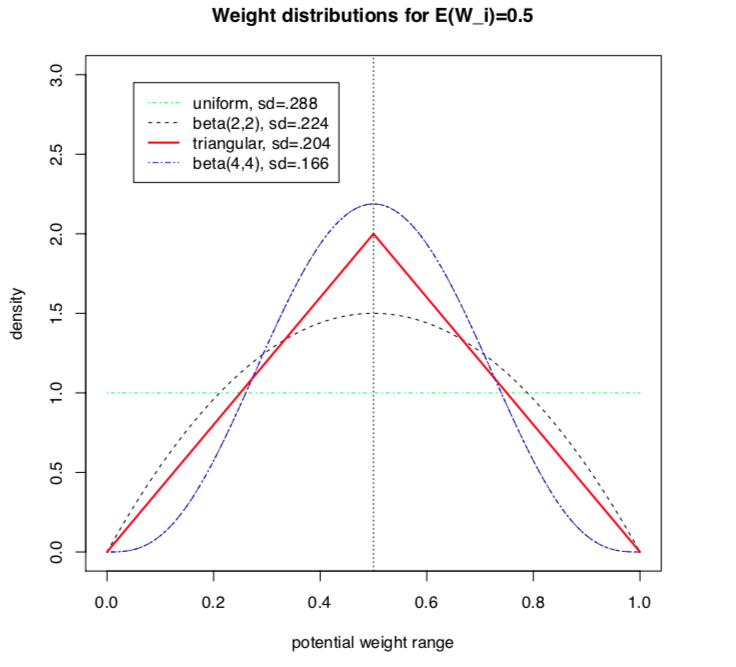
\includegraphics[width=\hsize]{Figures/18-1-weightDistributions.png}
\caption{Four models of uncertain criteria significance weights}
\label{fig:18.1}       % Give a unique label
\end{figure}

It is worthwhile noticing in Figure~\vref{fig:18.1} that these four uncertainty models all admit the same expected value, $E(W_j)$, however, with a respective variance which goes decreasing from $1/3$, to $1/9$ of the square of $E(W_j)$ \citep{BIS-2014}.

\section{Bipolar-valued likelihood of outranking situations}
\label{sec:18.2}

Let $A = \{x, y, z,...\}$ be a finite set of $n$ potential decision actions, evaluated on $F = \{1,..., m\}$ --a finite and coherent family of $m$ performance criteria. On each criterion $j \in F$, the decision actions are evaluated on a real performance scale $[0; M_j ]$, supporting an upper-closed indifference threshold $ind_j$ and a lower-closed preference threshold $pr_j$ such that $0 \leq ind_j < pr_j \leq M_j$. The marginal performance of object $x$ on criterion $j$ is denoted $x_j$. Each criterion $j$ is thus characterising a marginal double threshold order $\geq_j$ on $A$:
\begin{equation}
  r(x \geq_j y) \; = \; \begin{cases} +1 \quad \text{if} \quad x_j - y_j \leq -ind_j,\\  -1 \quad \text{if} \quad x_j - y_j \leq -pr_j,\\ 0 \quad \text{otherwise}. \end{cases}
\end{equation}

Semantics of the marginal bipolar-valued characteristic function:
\begin{itemize}[topsep=1pt]
\item $+1$ signifies $x$ is at least as well evaluated as $y$ on criterion $j$,
\item $-1$ signifies that $x$ is not at least as well evaluated as $y$ on criterion $j$,
\item $0$ signifies that it is unclear whether, on criterion $j$, $x$ is at least as well evaluated as $y$.
\end{itemize}
\begin{figure}[ht]
%\sidecaption
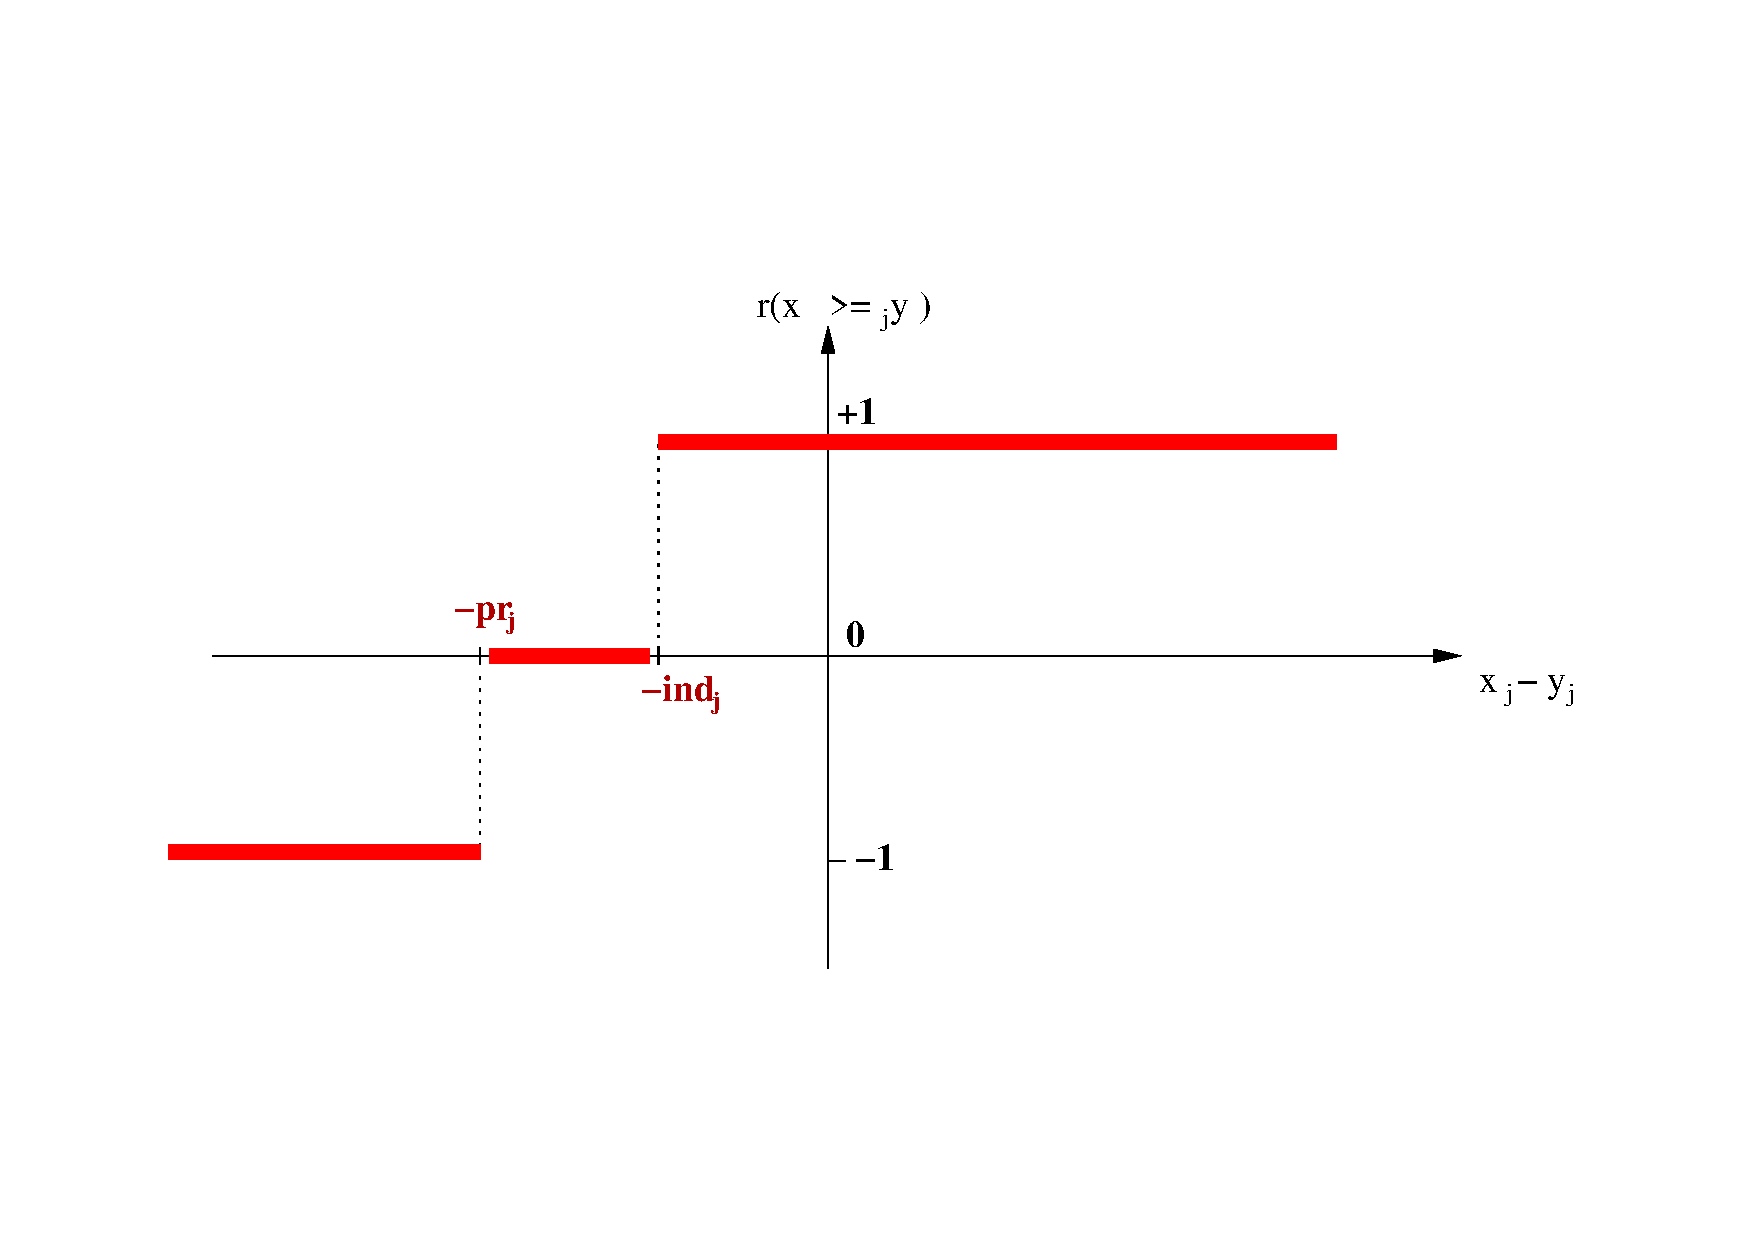
\includegraphics[width=\hsize]{Figures/18-2-rCharacteristic.pdf}
\caption{Bipolar-valued outranking characteristic function}
\label{fig:18.2}       % Give a unique label
\end{figure}

Each criterion $j$ in $F$ contributes the random significance $W_j$ of his ``\emph{at least as well evaluated as}'' characteristic $r(x \geq_j y)$ to the global characteristic $\tilde{r}(x \geq y)$ in the following way:
\begin{equation}
      \tilde{r}(x \geq y) \; = \; \sum_{j \in F} W_j \times r(x \geq_j y) )
\end{equation}

Thus, $\tilde{r}(x \geq y)$ becomes a simple sum of positive or negative independent random variables with known means and variances where $\tilde{r}(x \geq y) \, > \, 0$ signifies $x$ is globally at least as well evaluated as $y$, $\tilde{r}(x \geq y) \, < \, 0$ signifies that $x$ is not globally at least as well evaluated as $y$, and $\tilde{r}(x \geq y)\,=\,0$ signifies that it is unclear whether $x$ is globally at least as well evaluated as $y$.

From the \emph{Central Limit Theorem} (CLT), we know that such a sum of random variables leads, with $m$ getting large, to a Gaussian distribution $Y$ with
\begin{eqnarray}
E(Y ) = &\sum_{j \in F} \big(\,E(W_j) \times r(x \geq_j y)\,\big), \text{and}\\
V(Y) = &\sum_{j \in F} \big(\,V(W_j)\times |r(x \geq_j y)|\,\big).
\end{eqnarray}

And the \emph{likelihood of validation}, respectively \emph{invalidation} of an ``\emph{at least as well evaluated as}'' situation, denoted $lh(x \geq y)$,  may hence be assessed by the probability $P(Y > 0) = 1.0 - P(Y \leq 0)$ that $Y$ takes a positive, resp. $P(Y < 0)$ takes a negative value. In the bipolar-valued case here, we can judiciously make usage of the standard Gaussian \emph{error function} , i.e. the bipolar $2P(Z) - 1.0$ version of the standard Gaussian $P(Z)$ probability distribution function \citep{NR3-2007-6}:
\begin{equation}
  lh(x \geq y) \;=\; -\text{erf}\big(\frac{1}{\sqrt{2}}\frac{-E(Y)}{\sqrt{V(Y)}} \big)
\end{equation}

The range of the bipolar-valued $lh(x \geq y)$ hence becomes $[-1.0;+1.0]$, and $-lh(x \geq y) \,=\, lh(x \not\geq y)$ , i.e. a \emph{negative likelihood} represents the likelihood of the correspondent \emph{negated} ``\emph{at least as well evaluated as}'' situation. A likelihood of $+1.0$ (resp. $-1.0$) means the corresponding preferential situation appears \emph{certainly} validated (resp. invalidated).

\begin{example} Let $x$ and $y$ be evaluated with respect to 7 equisignificant criteria; Four criteria positively support that $x$ is \emph{as least as  well assessed as} $y$ and three criteria support that $x$ is \emph{not at least as well evaluated as} $y$. Suppose $E(W_j) = w$ for $j = 1,...,7$ and $W_j \leadsto Tr(0, 2w, w)$ for $j = 1,...7$. The expected value of the global ``\emph{at least as well evaluated as}'' characteristic value becomes: $E\big(\tilde{r}(x \geq y)\big)\, = \, 4w - 3w = w$ with a variance $V\big(\tilde{r}(x \geq y)\big)\,=\, 7\frac{1}{6}w^2$. 

If $w = 1$, $E\big(\tilde{r}(x \geq y)\big)\, = \, 1$ and $sd\big(\tilde{r}(x \geq y)\big)\,=\, 1.08$. By the CLT, the bipolar likelihood of the \emph{at least as well evaluated as} situation becomes: $lh(x \geq y)\,=\, 0.66$, which corresponds to a global support of $(0.66 + 1.0)/2 = 83\%$ of the criteria significance weights.

A \emph{Monte Carlo} simulation with $10\,000$ runs empirically confirms the effective convergence to a Gaussian (see Fig.~\vref{fig:18.3} realised with \emph{gretl}\footnote{The Gnu Regression, Econometrics and Time-series Library http://gretl.sourceforge.net/ .}).
\begin{figure}[ht]
%\sidecaption
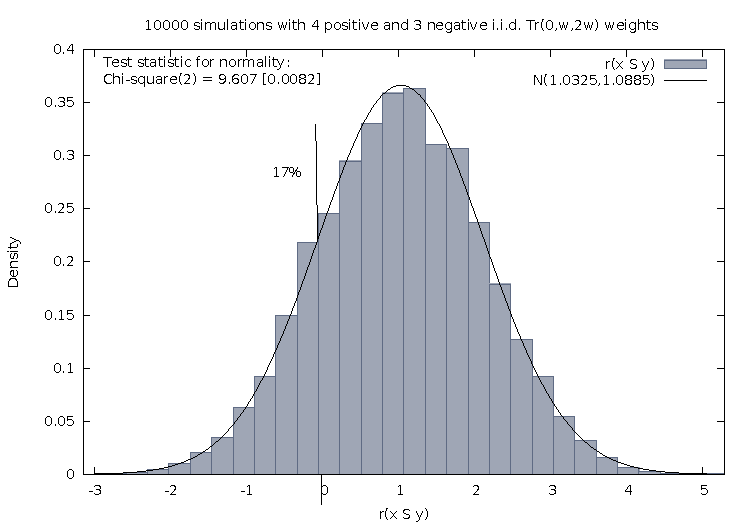
\includegraphics[width=\hsize]{Figures/18-3-simulLikelihood.pdf}
\caption{Distribution of $10\,000$ random outranking characteristic values.}
\label{fig:18.3}       % Give a unique label
\end{figure}

Indeed, $\tilde{r}(x \geq y) \leadsto Y = \mathcal{N}(1.03,1.089)$, with an empirical probability of observing a negative majority margin of about $17\%$.
\end{example}

\section{Confidence level of outranking digraphs}
\label{sec:18.3}

\begin{definition}[Confident outranking situation]\label{def:18.1}

\noindent Following the classical outranking approach (see \citep{BIS-2013}), we say, from an epistemic perspective, that decision action $x$ \emph{outranks} decision action $y$ at \emph{confidence} level $\alpha\%$, when:
\begin{itemize}[topsep=1pt]
\item An expected majority of criteria validates, at confidence level $\alpha\%$ or higher, a global ``\emph{at least as well evaluated as}'' situation between $x$ and $y$, and
\item no considerably less performing is observed on a discordant criterion.
\end{itemize}
Dually, decision action $x$ \emph{does not outrank} decision action $y$ at confidence level $\alpha\%$, when:
\begin{itemize}[topsep=0pt]
\item An expected minority only of criteria at confidence level $-\alpha\%$ or lesser, validates a global ``\emph{at least as well evaluated as}'' situation between $x$ and $y$, and
\item no considerably better performing situation is observed on a discordant criterion.
\end{itemize}
Otherwise, the situation is indeterminate.
\end{definition}

\noindent \textbf{Time for a coded example}

\noindent Let us consider the following random performance tableau.
\begin{lstlisting}[label=list:18.1,basicstyle=\ttfamily\scriptsize]
>>> from randomPerfTabs import RandomPerformanceTableau
>>> t = RandomPerformanceTableau(\
...          numberOfActions=7,\
...          numberOfCriteria=7,seed=100)
>>> t.showPerformanceTableau(Transposed=True)
  *----  performance tableau -----*
  criteria | weights |  'a1'   'a2'   'a3'   'a4'   'a5'   'a6'   'a7'   
  ---------|----------------------------------------------------------
     'g1'  |     1   | 15.17  44.51  57.87  58.00  24.22  29.10  96.58  
     'g2'  |     1   | 82.29  43.90    NA   35.84  29.12  34.79  62.22  
     'g3'  |     1   | 44.23  19.10  27.73  41.46  22.41  21.52  56.90  
     'g4'  |     1   | 46.37  16.22  21.53  51.16  77.01  39.35  32.06  
     'g5'  |     1   | 47.67  14.81  79.70  67.48    NA   90.72  80.16  
     'g6'  |     1   | 69.62  45.49  22.03  33.83  31.83    NA   48.80  
     'g7'  |     1   | 82.88  41.66  12.82  21.92  75.74  15.45   6.05  
\end{lstlisting}

For the corresponding confident outranking digraph, we assume uncertain criteria significance weights of \emph{triangular} distribution and require a confidence level of $\alpha = 90\%$. The \texttt{ConfidentBipolarOutrankingDigraph} class provides such a construction.
\begin{lstlisting}[label=list:18.2]
>>> from outrankingDigraphs import\
...        ConfidentBipolarOutrankingDigraph   
>>> g90 = ConfidentBipolarOutrankingDigraph(t,\
...        distribution ='triangular',confidence=90)
>>> g90
  *------- Object instance description ------*
   Instance class      : ConfidentBipolarOutrankingDigraph
   Instance name       : rel_randomperftab_CLT
   Actions           : 7
   Criteria          : 7
   Size                : 15
   Uncertainty model   : triangular(a=0,b=2w)
   Likelihood domain   : [-1.0;+1.0]
   Confidence level    : 0.80 (90.0%)
   Confident majority  : 0.14 (57.1%)
   Determinateness (%) : 62.07
   Valuation domain    : [-1.00;1.00]
   Attributes          : ['name', 'bipolarConfidenceLevel',
                 'distribution', 'betaParameter', 'actions',
                 'order', 'valuationdomain', 'criteria',
                 'evaluation', 'concordanceRelation',
                 'vetos', 'negativeVetos',
                 'largePerformanceDifferencesCount',
                 'likelihoods', 'confidenceCutLevel',
                 'relation', 'gamma', 'notGamma']
\end{lstlisting}

The resulting $90\%$-confident expected outranking relation is shown below.
\begin{lstlisting}[caption={$90\%$-confident outranking relation with triangular distributed significance weights},label=list:18.3,basicstyle=\ttfamily\scriptsize]
>>> g90.showRelationTable(LikelihoodDenotation=True)
  * ---- Outranking Relation Table -----
    r/(lh) |  'a1'    'a2'    'a3'    'a4'    'a5'    'a6'    'a7'	 
    -------|------------------------------------------------------
     'a1'  | +0.00   +0.71   +0.29   +0.29   +0.29   +0.29   +0.00  
           | ( - )  (+1.00) (+0.95) (+0.95) (+0.95) (+0.95) (+0.65) 
     'a2'  | -0.71   +0.00   -0.29   +0.00   +0.00   +0.29   -0.57  
           |(-1.00)  ( - )  (-0.95) (-0.65) (+0.73) (+0.95) (-1.00) 
     'a3'  | -0.29   +0.29   +0.00   -0.29   +0.00   +0.00   -0.29  
           |(-0.95) (+0.95)  ( - )  (-0.95) (-0.73) (-0.00) (-0.95) 
     'a4'  | +0.00   +0.00   +0.57   +0.00   +0.29   +0.57   -0.43  
       	   |(-0.00) (+0.65) (+1.00)  ( - )  (+0.95) (+1.00) (-0.99) 
     'a5'  | -0.29   +0.00   +0.00   +0.00   +0.00   +0.29   -0.29  
           |(-0.95) (-0.00) (+0.73) (-0.00)  ( - )  (+0.99) (-0.95) 
     'a6'  | -0.29   +0.00   +0.00   -0.29   +0.00   +0.00   +0.00  
           |(-0.95) (-0.00) (+0.73) (-0.95) (+0.73)  ( - )  (-0.00) 
     'a7'  | +0.00   +0.71   +0.57   +0.43   +0.29   +0.00   +0.00  
           |(-0.65) (+1.00) (+1.00) (+0.99) (+0.95) (-0.00)  ( - )  
    Valuation domain   : [-1.000; +1.000] 
    Uncertainty model  : triangular(a=2.0,b=2.0) 
    Likelihood domain  : [-1.0;+1.0] 
    Confidence level   : 0.80 (90.0%) 
    Confident majority : 0.14 (57.1%) 
    Determinateness    : 0.24 (62.1%)
\end{lstlisting}

The ($lh$) figures, indicated in Listing~\ref{list:18.3} above, correspond to bipolar likelihoods and the required bipolar confidence level equals $(0.90+1.0)/2 = 0.80$ (see Line 22 above). Action \texttt{a1} thus confidently outranks all other actions, except \texttt{a7} where the actual likelihood ($+0.65$) is lower than the required one ($+0.80$) and we furthermore observe a considerable counter-performance on criterion \texttt{g1}.

Notice also the lack of confidence in the outranking situations we observe between action \texttt{a2} and actions \texttt{a4} and \texttt{a5}. In the deterministic case we would have $r(a2 \geq a4) \,=\, -0.143$ and $r(a2 \geq a5) \,=\, +0.143$ . All outranking situations with a characteristic value lower or equal to $abs(0.143)$, i.e. a majority support of $1.143/2 = 57.1\%$ and less, appear indeed to be \emph{not confident} at $\alpha$ level $90\%$ (see Line 23 above).

Figure~\vref{fig:18.4} shows the corresponding strict $90\%$-confident outranking digraph, oriented by its initial and terminal strict prekernels.
\begin{lstlisting}
>>> gcd90 = ~ (-g90)
>>> gcd90.showPreKernels()
  *--- Computing preKernels ---*
   Dominant preKernels :
    ['a1', 'a7']
       independence :  0.0
       dominance    :  0.2857
       absorbency   :  -0.7143
       covering     :  0.800
   Absorbent preKernels :
    ['a2', 'a5', 'a6']
       independence :  0.0
       dominance    :  -0.2857
       absorbency   :  0.2857
       covered      :  0.583
>>> gcd90.exportGraphViz(fileName='confidentOutranking',
...        firstChoice=['a1', 'a7'],\
...        lastChoice=['a2', 'a5', 'a6'])
  *---- exporting a dot file for GraphViz tools ----*
   Exporting to confidentOutranking.dot
   dot -Grankdir=BT -Tpng confidentOutranking.dot\
                    -o confidentOutranking.png
\end{lstlisting}
\begin{figure}[ht]
\sidecaption[t]
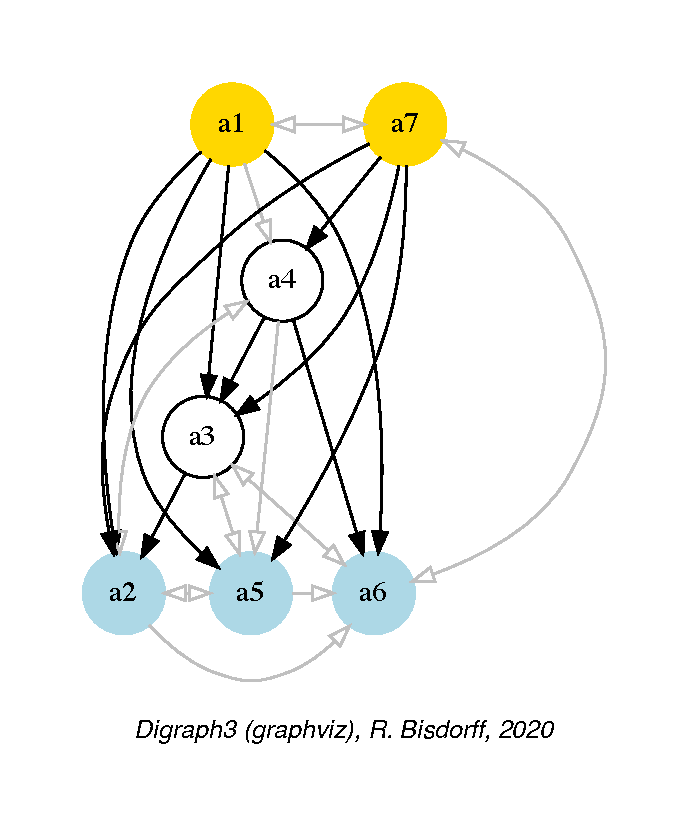
\includegraphics[width=7cm]{Figures/18-4-confidentOutranking.pdf}
\caption{90\%-confident strict outranking digraph oriented by its initial and terminal prekernels}
\label{fig:18.4}       % Give a unique label
\end{figure}

Now, what becomes this $90\%$-confident outranking digraph when we require a stronger confidence level of, say $99\%$?
\begin{lstlisting}[caption={$99\%$-confident outranking relation},label=list:18.4,basicstyle=\ttfamily\scriptsize]
>>> g99 = ConfidentBipolarOutrankingDigraph(t,\
...      distribution='trinagular',confidence=99)
>>> g99.showRelationTable()
  * ---- Outranking Relation Table -----
   r/(lh) |  'a1'    'a2'    'a3'    'a4'    'a5'    'a6'    'a7'	 
   -------|------------------------------------------------------
    'a1'  |  +0.00   +0.71   +0.00   +0.00   +0.00   +0.00   +0.00  
          |  ( - )  (+1.00) (+0.95) (+0.95) (+0.95) (+0.95) (+0.65) 
    'a2'  |  -0.71   +0.00   +0.00   +0.00   +0.00   +0.00   -0.57  
          | (-1.00)  ( - )  (-0.95) (-0.65) (+0.73) (+0.95) (-1.00) 
    'a3'  |  +0.00   +0.00   +0.00   +0.00   +0.00   +0.00   +0.00  
          | (-0.95) (+0.95)  ( - )  (-0.95) (-0.73) (-0.00) (-0.95) 
    'a4'  |  +0.00   +0.00   +0.57   +0.00   +0.00   +0.57   -0.43  
          | (-0.00) (+0.65) (+1.00)  ( - )  (+0.95) (+1.00) (-0.99) 
    'a5'  |  +0.00   +0.00   +0.00   +0.00   +0.00   +0.29   +0.00  
          | (-0.95) (-0.00) (+0.73) (-0.00)  ( - )  (+0.99) (-0.95) 
    'a6'  |  +0.00   +0.00   +0.00   +0.00   +0.00   +0.00   +0.00  
          | (-0.95) (-0.00) (+0.73) (-0.95) (+0.73)  ( - )  (-0.00) 
    'a7'  |  +0.00   +0.71   +0.57   +0.43   +0.00   +0.00   +0.00  
          | (-0.65) (+1.00) (+1.00) (+0.99) (+0.95) (-0.00)  ( - )  
    Valuation domain   : [-1.000; +1.000] 
    Uncertainty model  : triangular(a=0.0,b=2.0) 
    Likelihood domain  : [-1.0;+1.0] 
    Confidence level   : 0.98 (99.0%) 
    Confident majority : 0.29 (64.3%) 
    Determinateness    : 0.13 (56.6%)
\end{lstlisting}

At $99\%$ confidence, the minimal required significance majority support amounts to $64.3\%$ (see List.~\ref{list:18.4} Line 25 above). As a result, most outranking situations don't get anymore validated, like the outranking situations between action \texttt{a1} and actions \texttt{a3}, \texttt{a4}, \texttt{a5} and \texttt{a6} (see Line 5 above). The overall epistemic determination of the digraph consequently drops from $62.1\%$ to $56.6\%$ (see Line 26).

Finally, what becomes the previous $90\%$-confident outranking digraph when the uncertainty concerning the criteria significance weights is modelled with a larger variance, like \emph{uniform} variates (see Line 2 below).
\begin{lstlisting}[caption={$90\%$-confident outranking digraph with uniform variates},label=list:18.5, basicstyle=\ttfamily\scriptsize]
>>> gu90 = ConfidentBipolarOutrankingDigraph(t,\
...           confidence=90,distribution='uniform')
>>> gu90.showRelationTable()
  * ---- Outranking Relation Table -----
  r/(lh) |   'a1'    'a2'    'a3'    'a4'    'a5'    'a6'    'a7'	 
  -------|-------------------------------------------------------
    'a1' |  +0.00   +0.71   +0.29   +0.29   +0.29   +0.29   +0.00  
         |  ( - )  (+1.00) (+0.84) (+0.84) (+0.84) (+0.84) (+0.49) 
    'a2' |  -0.71   +0.00   -0.29   +0.00   +0.00   +0.29   -0.57  
         | (-1.00)  ( - )  (-0.84) (-0.49) (+0.56) (+0.84) (-1.00) 
    'a3' |  -0.29   +0.29   +0.00   -0.29   +0.00   +0.00   -0.29  
         | (-0.84) (+0.84)  ( - )  (-0.84) (-0.56) (-0.00) (-0.84) 
    'a4' |  +0.00   +0.00   +0.57   +0.00   +0.29   +0.57   -0.43  
         | (-0.00) (+0.49) (+1.00)  ( - )  (+0.84) (+1.00) (-0.95) 
    'a5' |  -0.29   +0.00   +0.00   +0.00   +0.00   +0.29   -0.29  
         | (-0.84) (-0.00) (+0.56) (-0.00)  ( - )  (+0.92) (-0.84) 
    'a6' |  -0.29   +0.00   +0.00   -0.29   +0.00   +0.00   +0.00  
         | (-0.84) (-0.00) (+0.56) (-0.84) (+0.56)  ( - )  (-0.00) 
    'a7' |  +0.00   +0.71   +0.57   +0.43   +0.29   +0.00   +0.00  
         | (-0.49) (+1.00) (+1.00) (+0.95) (+0.84) (-0.00)  ( - )  
    Valuation domain   : [-1.000; +1.000] 
    Uncertainty model  : uniform(a=0.0,b=2.0) 
    Likelihood domain  : [-1.0;+1.0] 
    Confidence level   : 0.80 (90.0%) 
    Confident majority : 0.14 (57.1%) 
    Determinateness    : 0.24 (62.1%)
\end{lstlisting}

Despite lower likelihood values (see the $g90$ digraph in List.~\vref{list:18.5}), we keep here the same confident majority level of $57.1\%$ (Line 25) and, hence, also the same $90\%$-confident outranking digraph.

For concluding, it is worthwhile noticing again that it is the \emph{neutral} value of the bipolar-valued epistemic logic that allows to easily handle $\alpha\%$ confidence or not of outranking situations when confronted with uncertain criteria significance weights. Remarkable furthermore is the usage, the standard Gaussian error function (erf) provides by delivering \emph{signed} likelihood values immediately concerning either a positive relational statement, or when negative, its negated version \citep{NR3-2007-6}. 
 
%%%%%%% The chapter bibliography
%\normallatexbib
\clearpage
%\phantomsection
%\addcontentsline{toc}{section}{Chapter Bibliography}
%\chapter[On confident outrankings]{On confident outrankings with uncertain criteria significance weights}
\label{sec:18}

\abstract*{When modelling preferences following the outranking approach, the signs of the majority margins do sharply distribute validation and invalidation of pairwise outranking situations. How can we be confident in the resulting outranking digraph, when we acknowledge the usual imprecise knowledge of criteria significance weights coupled with small majority margins? To answer this question, one usually requires \emph{qualified} majority margins for confirming outranking situations. But how to choose such a qualifying majority level: two third, three fourth of the significances ? In this chapter we propose to link the qualifying significance majority with a required $\alpha\%$-confidence level. We model therefore the significance weights as random variables following more or less widespread distributions around an average significance value that corresponds to the given deterministic weight. As the bipolar-valued random credibility of an outranking statement hence results from the simple sum of positive or negative independent random variables, we may apply the Central Limit Theorem (CLT) for computing the bipolar likelihood that the expected majority margin will indeed be positive, respectively negative.}

\abstract{When modelling preferences following the outranking approach, the signs of the majority margins do sharply distribute validation and invalidation of pairwise outranking situations. How can we be confident in the resulting outranking digraph, when we acknowledge the usual imprecise knowledge of criteria significance weights coupled with small majority margins? To answer this question, one usually requires \emph{qualified} majority margins for confirming outranking situations. But how to choose such a qualifying majority level: two third, three fourth of the significances ? In this chapter we propose to link the qualifying significance majority with a required $\alpha\%$-confidence level. We model therefore the significance weights as random variables following more or less widespread distributions around an average significance value that corresponds to the given deterministic weight. As the bipolar-valued random credibility of an outranking statement hence results from the simple sum of positive or negative independent random variables, we may apply the Central Limit Theorem (CLT) for computing the bipolar likelihood that the expected majority margin will indeed be positive, respectively negative.}

\section{Modelling uncertain criteria significances}
\label{sec:18.1}

Let us consider the significance weights of a family $F$ of $m$ criteria to be independent random variables $W_j$, distributing the potential significance weights of each criterion $j = 1, ..., m$ around a mean value $E(W_j)$ with variance $V(W_j)$.

Choosing a specific stochastic model of uncertainty is usually application specific. In the limited scope of this chapter, we will illustrate the consequence of this design decision on the resulting outranking modelling with four slightly different models for taking into account the uncertainty with which we know the numerical significance weights: \emph{uniform}, \emph{triangular}, and two models of \emph{Beta laws}, one more widespread and, the other, more concentrated.

When considering, for instance, that the potential range of a significance weight is distributed between $0$ and two times its mean value, we obtain the following random variates:
\begin{itemize}
\item A continuous \emph{uniform} distribution on the range $0$ to $2E(W_j)$. Thus $W_j \leadsto U(0, 2E(W_j))$ and $V(W_j) = 1/3(E(W_j))^2$;
\item A \emph{symmetric beta} distribution with, for instance, parameters  $\alpha = 2$ and $\beta = 2$. Thus, $W_i \leadsto Beta(2,2) \times 2E(W_j)$ and $V(W_j) = 1/5(E(Wj))^2$;
\item A \emph{symmetric triangular} distribution on the same range wit mode $E(W_j)$. Thus $W_j \leadsto Tr(0, 2E(W_j), E(Wj))$ with $V(W_j) = 1/6(E(Wj))^2$;
\item A \emph{narrower beta} distribution with, for instance, parameters $\alpha = 4$ and $\beta = 4$. Thus $W_j \leadsto Beta(4,4) \times 2E(W_j)$ , $V(W_j) = 1/9(E(W_j))^2$.
\end{itemize}
\begin{figure}[h]
%\sidecaption
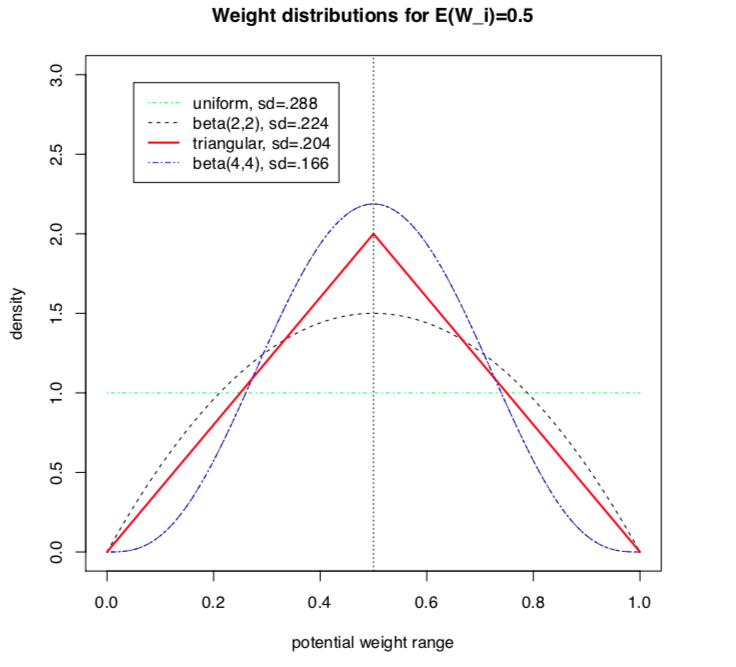
\includegraphics[width=12cm]{Figures/weightDistributions.png}
\caption{Four models of uncertain significance weights}
\label{fig:18.1}       % Give a unique label
\end{figure}
It is worthwhile noticing that these four uncertainty models all admit the same expected value, $E(W_j)$, however, with a respective variance which goes decreasing from $1/3$, to $1/9$ of the square of $E(W_j)$ (see Fig. \ref{fig:18.1}).

\section{Bipolar-valued likelihood of outranking situations}
\label{sec:18.2}

Let $A = \{x, y, z,...\}$ be a finite set of $n$ potential decision actions, evaluated on $F = \{1,..., m\}$ --a finite and coherent family of $m$ performance criteria. On each criterion $j \in F$, the decision actions are evaluated on a real performance scale $[0; M_j ]$, supporting an upper-closed indifference threshold $indj$ and a lower-closed preference threshold $prj$ such that $0 \leq indj < prj \leq M_j$. The marginal performance of object $x$ on criterion $j$ is denoted $x_j$. Each criterion $j$ is thus characterising a marginal double threshold order $\geq_j$ on $A$:
\begin{equation}
  r(x \geq_j y) \; = \; \begin{cases} +1 \quad \text{if} \quad x_j - y_j \leq -ind_j,\\  -1 \quad \text{if} \quad x_j - y_j \leq -pr_j,\\ 0 \quad \text{otherwise}. \end{cases}
\end{equation}

Semantics of the marginal bipolar-valued characteristic function:
\begin{itemize}
\item $+1$ signifies $x$ is performing at least as good as $y$ on criterion $j$,
\item $-1$ signifies that $x$ is not performing at least as good as $y$ on criterion $j$,
\item $0$ signifies that it is unclear whether, on criterion $j$, $x$ is performing at least as good as $y$.
\end{itemize}
\begin{figure}[h]
%\sidecaption
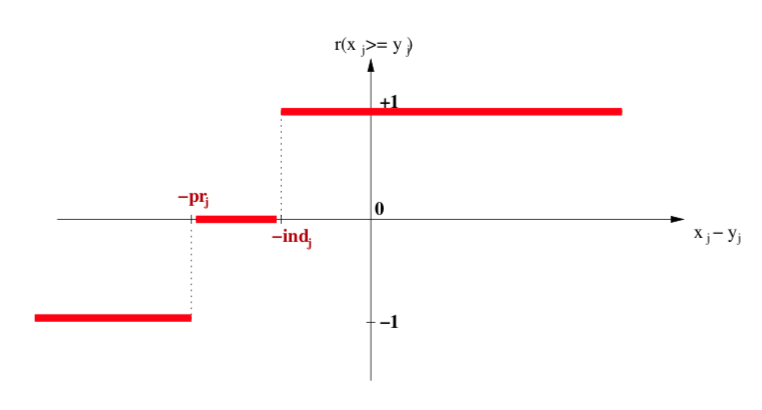
\includegraphics[width=11cm]{Figures/rCharacteristic.png}
\caption{Bipolar-valued outranking characteristic function.}
\label{fig:18.2}       % Give a unique label
\end{figure}
Each criterion $j$ in $F$ contributes the random significance $W_j$ of his ``\emph{at least as good as}'' characteristic $r(x \geq_j y)$ to the global characteristic $\tilde{r}(x \geq y)$ in the following way:
\begin{equation}
      \tilde{r}(x \geq y) \; = \; \sum_{j \in F} W_j \times r(x \geq_j y) )
    \end{equation}
Thus, $\tilde{r}(x \geq y)$ becomes a simple sum of positive or negative independent random variables with known means and variances where $\tilde{r}(x \geq y) \, > \, 0$ signifies $x$ is globally performing at least as good as $y$, $\tilde{r}(x \geq y) \, < \, 0$ signifies that $x$ is not globally performing at least as good as $y$, and $\tilde{r}(x \geq y)\,=\,0$ signifies that it is unclear whether $x$ is globally performing at least as good as $y$.

From the \emph{Central Limit Theorem} (CLT), we know that such a sum of random variables leads, with $m$ getting large, to a Gaussian distribution $Y$ with
\begin{eqnarray}
E(Y ) = &\sum_{j \in F} \big(\,E(W_j) \times r(x \geq_j y)\,\big), \text{and}\\
V(Y) = &\sum_{j \in F} \big(\,V(W_j)\times |r(x \geq_j y)|\,\big).
\end{eqnarray}
And the \emph{likelihood of validation}, respectively \emph{invalidation} of an ``\emph{at least as good as}'' situation, denoted $lh(x \geq y)$,  may hence be assessed by the probability $P(Y > 0) = 1.0 - P(Y \leq 0)$ that $Y$ takes a positive, resp. $P(Y < 0)$ takes a negative value. In the bipolar-valued case here, we can judiciously make usage of the standard Gaussian \emph{error function} , i.e. the bipolar $2P(Z) - 1.0$ version of the standard Gaussian $P(Z)$ probability distribution function:
\begin{equation}
  lh(x \geq y) \;=\; -\text{erf}\big(\frac{1}{\sqrt{2}}\frac{-E(Y)}{\sqrt{V(Y)}} \big)
\end{equation}
The range of the bipolar-valued $lh(x \geq y)$ hence becomes $[-1.0;+1.0]$, and $-lh(x \geq y) \,=\, lh(x \not\geq y)$ , i.e. a \emph{negative likelihood} represents the likelihood of the correspondent \emph{negated} ``\emph{at least as good as}'' situation. A likelihood of $+1.0$ (resp. $-1.0$) means the corresponding preferential situation appears \emph{certainly} validated (resp. invalidated).

\begin{example} Let $x$ and $y$ be evaluated wrt 7 equisignificant criteria; Four criteria positively support that $x$ is \emph{as least as good performing} than $y$ and three criteria support that $x$ is \emph{not at least as good} performing than $y$. Suppose $E(W_j) = w$ for $j = 1,...,7$ and $W_j \leadsto Tr(0, 2w, w)$ for $j = 1,...7$. The expected value of the global ``\emph{at least as good as}'' characteristic value becomes: $E\big(\tilde{r}(x \geq y)\big)\, = \, 4w - 3w = w$ with a variance $V\big(\tilde{r}(x \geq y)\big)\,=\, 7\frac{1}{6}w^2$. 

If $w = 1$, $E\big(\tilde{r}(x \geq y)\big)\, = \, 1$ and $sd\big(\tilde{r}(x \geq y)\big)\,=\, 1.08$. By the CLT, the bipolar likelihood of the \emph{at least as good} performing situation becomes: $lh(x \geq y)\,=\, 0.66$, which corresponds to a global support of $(0.66 + 1.0)/2 = 83\%$ of the criteria significance weights.

A \emph{Monte Carlo} simulation with $10\,000$ runs empirically confirms the effective convergence to a Gaussian (see Fig. \ref{fig:18.3} realised with \emph{gretl} \footnote{The Gnu Regression, Econometrics and Time-series Library http://gretl.sourceforge.net/ .}.
\begin{figure}[h]
%\sidecaption
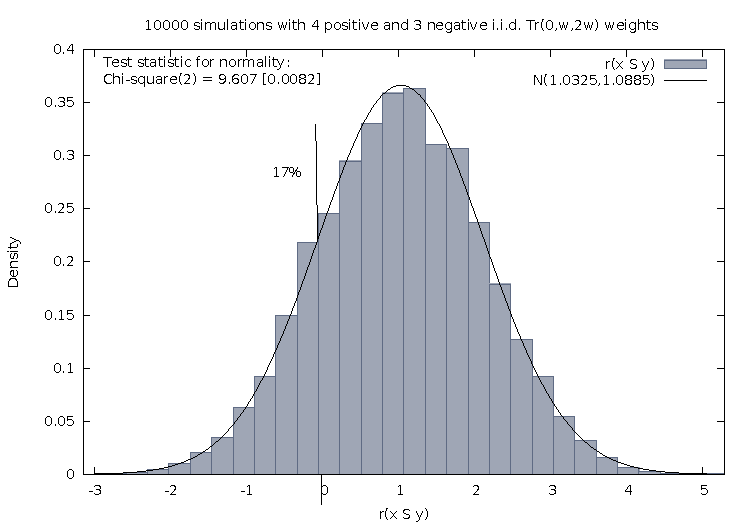
\includegraphics[width=12cm]{Figures/simulLikelihood.pdf}
\caption{Distribution of $10\,000$ random outranking characteristic values.}
\label{fig:18.3}       % Give a unique label
\end{figure}
Indeed, $\tilde{r}(x \geq y) \leadsto Y = \mathcal{N}(1.03,1.089)$, with an empirical probability of observing a negative majority margin of about $17\%$.
\end{example}

\section{Confidence level of outranking digraphs}
\label{sec:18.3}

Now, following the classical outranking approach (see \citep{BIS-2013}), we may say, from an epistemic perspective, that decision action $x$ \emph{outranks} decision action $y$ at \emph{confidence} level $\alpha \%$, when
\begin{itemize}
\item An expected majority of criteria validates, at confidence level $\alpha \%$ or higher, a global ``\emph{at least as good as}'' situation between $x$ and $y$, and
\item no considerably less performing is observed on a discordant criterion.
\end{itemize}
Dually, decision action $x$ \emph{does not outrank} decision action $y$ at
confidence level $\alpha \%$, when
\begin{itemize}
\item An expected majority of criteria at confidence level $\alpha \%$ or higher, invalidates a global ``\emph{at least as good as}'' situation between $x$ and $y$, and
\item no considerably better performing situation is observed on a discordant criterion.
\end{itemize}

\noindent \textbf{Time for a coded example}
Let us consider the following random performance tableau.
\begin{lstlisting}[basicstyle=\scriptsize]
>>> from randomPerfTabs import RandomPerformanceTableau
>>> t = RandomPerformanceTableau(\
...          numberOfActions=7,\
...          numberOfCriteria=7,seed=100)
>>> t.showPerformanceTableau(Transposed=True)
  *----  performance tableau -----*
  criteria | weights |  'a1'   'a2'   'a3'   'a4'   'a5'   'a6'   'a7'   
  ---------|----------------------------------------------------------
     'g1'  |     1   | 15.17  44.51  57.87  58.00  24.22  29.10  96.58  
     'g2'  |     1   | 82.29  43.90    NA   35.84  29.12  34.79  62.22  
     'g3'  |     1   | 44.23  19.10  27.73  41.46  22.41  21.52  56.90  
     'g4'  |     1   | 46.37  16.22  21.53  51.16  77.01  39.35  32.06  
     'g5'  |     1   | 47.67  14.81  79.70  67.48    NA   90.72  80.16  
     'g6'  |     1   | 69.62  45.49  22.03  33.83  31.83    NA   48.80  
     'g7'  |     1   | 82.88  41.66  12.82  21.92  75.74  15.45   6.05  
\end{lstlisting}

For the corresponding confident outranking digraph, we require a confidence level of $\alpha = 90\%$.

The \texttt{ConfidentBipolarOutrankingDigraph} class provides such a construction.
\begin{lstlisting}
>>> from outrankingDigraphs import\
...        ConfidentBipolarOutrankingDigraph   
>>> g90 = ConfidentBipolarOutrankingDigraph(t,confidence=90)
>>> g90
  *------- Object instance description ------*
   Instance class      : ConfidentBipolarOutrankingDigraph
   Instance name       : rel_randomperftab_CLT
   Actions           : 7
   Criteria          : 7
   Size                : 15
   Uncertainty model   : triangular(a=0,b=2w)
   Likelihood domain   : [-1.0;+1.0]
   Confidence level    : 0.80 (90.0%)
   Confident majority  : 0.14 (57.1%)
   Determinateness (%) : 62.07
   Valuation domain    : [-1.00;1.00]
   Attributes          : ['name', 'bipolarConfidenceLevel',
                 'distribution', 'betaParameter', 'actions',
                 'order', 'valuationdomain', 'criteria',
                 'evaluation', 'concordanceRelation',
                 'vetos', 'negativeVetos',
                 'largePerformanceDifferencesCount',
                 'likelihoods', 'confidenceCutLevel',
                 'relation', 'gamma', 'notGamma']
\end{lstlisting}

The resulting $90\%$-confident expected outranking relation is shown below.
\begin{lstlisting}[basicstyle=\scriptsize]
>>> g90.showRelationTable(LikelihoodDenotation=True)
  * ---- Outranking Relation Table -----
    r/(lh) |  'a1'    'a2'    'a3'    'a4'    'a5'    'a6'    'a7'	 
    -------|------------------------------------------------------
     'a1'  | +0.00   +0.71   +0.29   +0.29   +0.29   +0.29   +0.00  
           | ( - )  (+1.00) (+0.95) (+0.95) (+0.95) (+0.95) (+0.65) 
     'a2'  | -0.71   +0.00   -0.29   +0.00   +0.00   +0.29   -0.57  
           |(-1.00)  ( - )  (-0.95) (-0.65) (+0.73) (+0.95) (-1.00) 
     'a3'  | -0.29   +0.29   +0.00   -0.29   +0.00   +0.00   -0.29  
           |(-0.95) (+0.95)  ( - )  (-0.95) (-0.73) (-0.00) (-0.95) 
     'a4'  | +0.00   +0.00   +0.57   +0.00   +0.29   +0.57   -0.43  
       	   |(-0.00) (+0.65) (+1.00)  ( - )  (+0.95) (+1.00) (-0.99) 
     'a5'  | -0.29   +0.00   +0.00   +0.00   +0.00   +0.29   -0.29  
           |(-0.95) (-0.00) (+0.73) (-0.00)  ( - )  (+0.99) (-0.95) 
     'a6'  | -0.29   +0.00   +0.00   -0.29   +0.00   +0.00   +0.00  
           |(-0.95) (-0.00) (+0.73) (-0.95) (+0.73)  ( - )  (-0.00) 
     'a7'  | +0.00   +0.71   +0.57   +0.43   +0.29   +0.00   +0.00  
           |(-0.65) (+1.00) (+1.00) (+0.99) (+0.95) (-0.00)  ( - )  
    Valuation domain   : [-1.000; +1.000] 
    Uncertainty model  : triangular(a=2.0,b=2.0) 
    Likelihood domain  : [-1.0;+1.0] 
    Confidence level   : 0.80 (90.0%) 
    Confident majority : 0.14 (57.1%) 
    Determinateness    : 0.24 (62.1%)
\end{lstlisting}

The ($lh$) figures, indicated in the table above, correspond to bipolar likelihoods and the required bipolar confidence level equals $(0.90+1.0)/2 = 0.80$ (see Line 22 above). Action 'a1' thus confidently outranks all other actions, except 'a7' where the actual likelihood ($+0.65$) is lower than the required one ($0.80$) and we furthermore observe a considerable counter-performance on criterion 'g1'.

Notice also the lack of confidence in the outranking situations we observe between action 'a2' and actions 'a4' and 'a5'. In the deterministic case we would have $r(a2 \geq a4) \,=\, -0.143$ and $r(a2 \geq a5) \,=\, +0.143$ . All outranking situations with a characteristic value lower or equal to $abs(0.143)$, i.e. a majority support of $1.143/2 = 57.1\%$ and less, appear indeed to be \emph{not confident} at $\alpha$ level $90\%$ (see Line 23 above).

We may draw the corresponding strict $90\%$-confident outranking digraph, oriented by its initial and terminal strict prekernels (see Fig. \ref{fig:18.4}).
\begin{lstlisting}
>>> gcd90 = ~ (-g90)
>>> gcd90.showPreKernels()
  *--- Computing preKernels ---*
   Dominant preKernels :
    ['a1', 'a7']
       independence :  0.0
       dominance    :  0.2857
       absorbency   :  -0.7143
       covering     :  0.800
   Absorbent preKernels :
    ['a2', 'a5', 'a6']
       independence :  0.0
       dominance    :  -0.2857
       absorbency   :  0.2857
       covered      :  0.583
>>> gcd90.exportGraphViz(fileName='confidentOutranking',
...        bestChoice=['a1', 'a7'],worstChoice=['a2', 'a5', 'a6'])
  *---- exporting a dot file for GraphViz tools ---------*
   Exporting to confidentOutranking.dot
   dot -Grankdir=BT -Tpng confidentOutranking.dot\
                    -o confidentOutranking.png
\end{lstlisting}

\begin{figure}[h]
\sidecaption
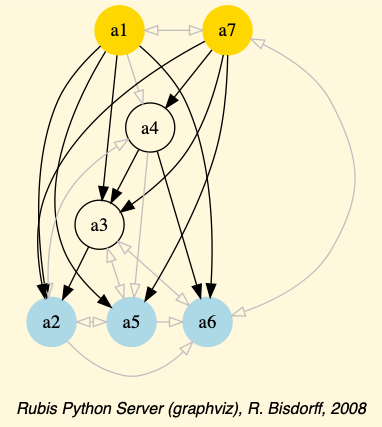
\includegraphics[width=6cm]{Figures/confidentOutranking.png}
\caption{90\%-confident strict outranking digraph oriented by its prekernels}
\label{fig:18.4}       % Give a unique label
\end{figure}

Now, what becomes this 90\%-confident outranking digraph when we require a stronger confidence level of, say $99\%$?
\begin{lstlisting}[basicstyle=\scriptsize]
>>> g99 = ConfidentBipolarOutrankingDigraph(t,confidence=99)
>>> g99.showRelationTable()
  * ---- Outranking Relation Table -----
   r/(lh) |  'a1'    'a2'    'a3'    'a4'    'a5'    'a6'    'a7'	 
   -------|------------------------------------------------------
    'a1'  |  +0.00   +0.71   +0.00   +0.00   +0.00   +0.00   +0.00  
          |  ( - )  (+1.00) (+0.95) (+0.95) (+0.95) (+0.95) (+0.65) 
    'a2'  |  -0.71   +0.00   +0.00   +0.00   +0.00   +0.00   -0.57  
          | (-1.00)  ( - )  (-0.95) (-0.65) (+0.73) (+0.95) (-1.00) 
    'a3'  |  +0.00   +0.00   +0.00   +0.00   +0.00   +0.00   +0.00  
          | (-0.95) (+0.95)  ( - )  (-0.95) (-0.73) (-0.00) (-0.95) 
    'a4'  |  +0.00   +0.00   +0.57   +0.00   +0.00   +0.57   -0.43  
          | (-0.00) (+0.65) (+1.00)  ( - )  (+0.95) (+1.00) (-0.99) 
    'a5'  |  +0.00   +0.00   +0.00   +0.00   +0.00   +0.29   +0.00  
          | (-0.95) (-0.00) (+0.73) (-0.00)  ( - )  (+0.99) (-0.95) 
    'a6'  |  +0.00   +0.00   +0.00   +0.00   +0.00   +0.00   +0.00  
          | (-0.95) (-0.00) (+0.73) (-0.95) (+0.73)  ( - )  (-0.00) 
    'a7'  |  +0.00   +0.71   +0.57   +0.43   +0.00   +0.00   +0.00  
          | (-0.65) (+1.00) (+1.00) (+0.99) (+0.95) (-0.00)  ( - )  
    Valuation domain   : [-1.000; +1.000] 
    Uncertainty model  : triangular(a=2.0,b=2.0) 
    Likelihood domain  : [-1.0;+1.0] 
    Confidence level   : 0.98 (99.0%) 
    Confident majority : 0.29 (64.3%) 
    Determinateness    : 0.13 (56.6%)
\end{lstlisting}

At $99\%$ confidence, the minimal required significance majority support amounts to $64.3\%$ (see Line 24 above). As a result, most outranking situations don't get anymore validated, like the outranking situations between action 'a1' and actions 'a3', 'a4', 'a5' and 'a6' (see Line 5 above). The overall epistemic determination of the digraph consequently drops from $.1\%$ to $56.6\%$ (see Line 25).

Finally, what becomes the previous $90\%$-confident outranking digraph if the uncertainty concerning the criteria significance weights is modelled with a larger variance, like \emph{uniform} variates (see Line 2 below).
\begin{lstlisting}[basicstyle=\scriptsize]
>>> gu90 = ConfidentBipolarOutrankingDigraph(t,\
...           confidence=90,distribution='uniform')
>>> gu90.showRelationTable()
  * ---- Outranking Relation Table -----
  r/(lh) |   'a1'    'a2'    'a3'    'a4'    'a5'    'a6'    'a7'	 
  -------|-------------------------------------------------------
    'a1' |  +0.00   +0.71   +0.29   +0.29   +0.29   +0.29   +0.00  
         |  ( - )  (+1.00) (+0.84) (+0.84) (+0.84) (+0.84) (+0.49) 
    'a2' |  -0.71   +0.00   -0.29   +0.00   +0.00   +0.29   -0.57  
         | (-1.00)  ( - )  (-0.84) (-0.49) (+0.56) (+0.84) (-1.00) 
    'a3' |  -0.29   +0.29   +0.00   -0.29   +0.00   +0.00   -0.29  
         | (-0.84) (+0.84)  ( - )  (-0.84) (-0.56) (-0.00) (-0.84) 
    'a4' |  +0.00   +0.00   +0.57   +0.00   +0.29   +0.57   -0.43  
         | (-0.00) (+0.49) (+1.00)  ( - )  (+0.84) (+1.00) (-0.95) 
    'a5' |  -0.29   +0.00   +0.00   +0.00   +0.00   +0.29   -0.29  
         | (-0.84) (-0.00) (+0.56) (-0.00)  ( - )  (+0.92) (-0.84) 
    'a6' |  -0.29   +0.00   +0.00   -0.29   +0.00   +0.00   +0.00  
         | (-0.84) (-0.00) (+0.56) (-0.84) (+0.56)  ( - )  (-0.00) 
    'a7' |  +0.00   +0.71   +0.57   +0.43   +0.29   +0.00   +0.00  
         | (-0.49) (+1.00) (+1.00) (+0.95) (+0.84) (-0.00)  ( - )  
    Valuation domain   : [-1.000; +1.000] 
    Uncertainty model  : uniform(a=2.0,b=2.0) 
    Likelihood domain  : [-1.0;+1.0] 
    Confidence level   : 0.80 (90.0%) 
    Confident majority : 0.14 (57.1%) 
    Determinateness    : 0.24 (62.1%)
\end{lstlisting}

Despite lower likelihood values (see the $g90$ relation table above), we keep the same confident majority level of $57.1\%$ (see Line 25 above) and, hence, also the same $90\%$-confident outranking digraph.

For concluding, it is worthwhile noticing again that it is in fact the \emph{neutral} value of our bipolar-valued epistemic logic that allows us to easily handle $\alpha\%$ confidence or not of outranking situations when confronted with uncertain criteria significances. Remarkable furthermore is the usage, the standard Gaussian error function (erf) provides by delivering \emph{signed} likelihood values immediately concerning either a positive relational statement, or when negative, its negated version. 
 
%%%%%%% The chapter bibliography
%\normallatexbib
\clearpage
%\phantomsection
%\addcontentsline{toc}{section}{Chapter Bibliography}
\bibliographystyle{spbasic}
%\typeout{}
\bibliography{03-backMatters/reference}
%\chapter[On confident outrankings]{On confident outrankings with uncertain criteria significance weights}
\label{sec:18}

\abstract*{When modelling preferences following the outranking approach, the signs of the majority margins do sharply distribute validation and invalidation of pairwise outranking situations. How can we be confident in the resulting outranking digraph, when we acknowledge the usual imprecise knowledge of criteria significance weights coupled with small majority margins? To answer this question, one usually requires \emph{qualified} majority margins for confirming outranking situations. But how to choose such a qualifying majority level: two third, three fourth of the significances ? In this chapter we propose to link the qualifying significance majority with a required $\alpha\%$-confidence level. We model therefore the significance weights as random variables following more or less widespread distributions around an average significance value that corresponds to the given deterministic weight. As the bipolar-valued random credibility of an outranking statement hence results from the simple sum of positive or negative independent random variables, we may apply the Central Limit Theorem (CLT) for computing the bipolar likelihood that the expected majority margin will indeed be positive, respectively negative.}

\abstract{When modelling preferences following the outranking approach, the signs of the majority margins do sharply distribute validation and invalidation of pairwise outranking situations. How can we be confident in the resulting outranking digraph, when we acknowledge the usual imprecise knowledge of criteria significance weights coupled with small majority margins? To answer this question, one usually requires \emph{qualified} majority margins for confirming outranking situations. But how to choose such a qualifying majority level: two third, three fourth of the significances ? In this chapter we propose to link the qualifying significance majority with a required $\alpha\%$-confidence level. We model therefore the significance weights as random variables following more or less widespread distributions around an average significance value that corresponds to the given deterministic weight. As the bipolar-valued random credibility of an outranking statement hence results from the simple sum of positive or negative independent random variables, we may apply the Central Limit Theorem (CLT) for computing the bipolar likelihood that the expected majority margin will indeed be positive, respectively negative.}

\section{Modelling uncertain criteria significances}
\label{sec:18.1}

Let us consider the significance weights of a family $F$ of $m$ criteria to be independent random variables $W_j$, distributing the potential significance weights of each criterion $j = 1, ..., m$ around a mean value $E(W_j)$ with variance $V(W_j)$.

Choosing a specific stochastic model of uncertainty is usually application specific. In the limited scope of this chapter, we will illustrate the consequence of this design decision on the resulting outranking modelling with four slightly different models for taking into account the uncertainty with which we know the numerical significance weights: \emph{uniform}, \emph{triangular}, and two models of \emph{Beta laws}, one more widespread and, the other, more concentrated.

When considering, for instance, that the potential range of a significance weight is distributed between $0$ and two times its mean value, we obtain the following random variates:
\begin{itemize}
\item A continuous \emph{uniform} distribution on the range $0$ to $2E(W_j)$. Thus $W_j \leadsto U(0, 2E(W_j))$ and $V(W_j) = 1/3(E(W_j))^2$;
\item A \emph{symmetric beta} distribution with, for instance, parameters  $\alpha = 2$ and $\beta = 2$. Thus, $W_i \leadsto Beta(2,2) \times 2E(W_j)$ and $V(W_j) = 1/5(E(Wj))^2$;
\item A \emph{symmetric triangular} distribution on the same range wit mode $E(W_j)$. Thus $W_j \leadsto Tr(0, 2E(W_j), E(Wj))$ with $V(W_j) = 1/6(E(Wj))^2$;
\item A \emph{narrower beta} distribution with, for instance, parameters $\alpha = 4$ and $\beta = 4$. Thus $W_j \leadsto Beta(4,4) \times 2E(W_j)$ , $V(W_j) = 1/9(E(W_j))^2$.
\end{itemize}
\begin{figure}[h]
%\sidecaption
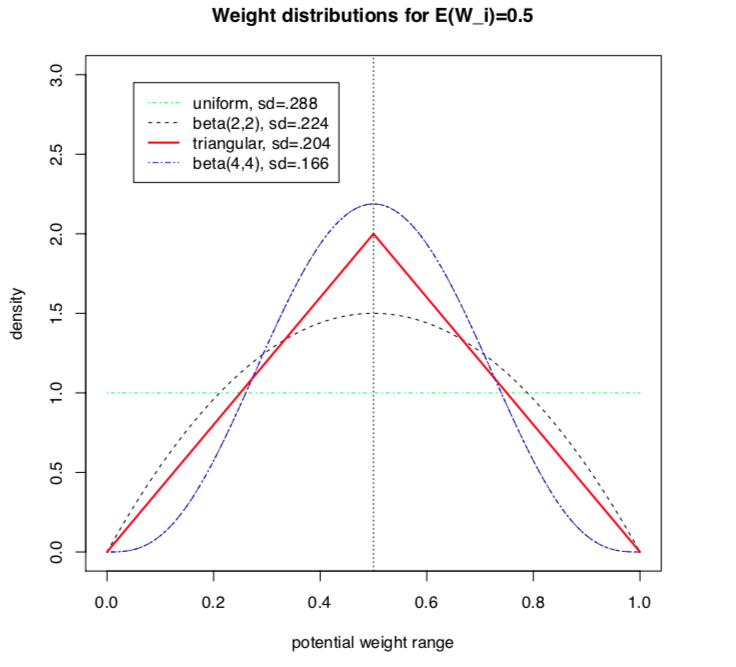
\includegraphics[width=12cm]{Figures/weightDistributions.png}
\caption{Four models of uncertain significance weights}
\label{fig:18.1}       % Give a unique label
\end{figure}
It is worthwhile noticing that these four uncertainty models all admit the same expected value, $E(W_j)$, however, with a respective variance which goes decreasing from $1/3$, to $1/9$ of the square of $E(W_j)$ (see Fig. \ref{fig:18.1}).

\section{Bipolar-valued likelihood of outranking situations}
\label{sec:18.2}

Let $A = \{x, y, z,...\}$ be a finite set of $n$ potential decision actions, evaluated on $F = \{1,..., m\}$ --a finite and coherent family of $m$ performance criteria. On each criterion $j \in F$, the decision actions are evaluated on a real performance scale $[0; M_j ]$, supporting an upper-closed indifference threshold $indj$ and a lower-closed preference threshold $prj$ such that $0 \leq indj < prj \leq M_j$. The marginal performance of object $x$ on criterion $j$ is denoted $x_j$. Each criterion $j$ is thus characterising a marginal double threshold order $\geq_j$ on $A$:
\begin{equation}
  r(x \geq_j y) \; = \; \begin{cases} +1 \quad \text{if} \quad x_j - y_j \leq -ind_j,\\  -1 \quad \text{if} \quad x_j - y_j \leq -pr_j,\\ 0 \quad \text{otherwise}. \end{cases}
\end{equation}

Semantics of the marginal bipolar-valued characteristic function:
\begin{itemize}
\item $+1$ signifies $x$ is performing at least as good as $y$ on criterion $j$,
\item $-1$ signifies that $x$ is not performing at least as good as $y$ on criterion $j$,
\item $0$ signifies that it is unclear whether, on criterion $j$, $x$ is performing at least as good as $y$.
\end{itemize}
\begin{figure}[h]
%\sidecaption
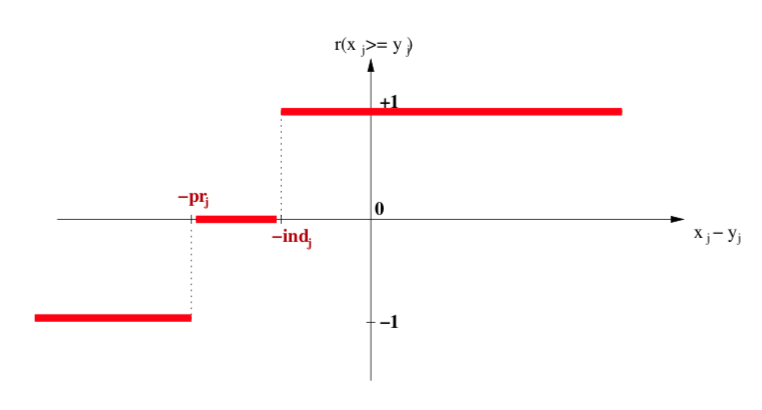
\includegraphics[width=11cm]{Figures/rCharacteristic.png}
\caption{Bipolar-valued outranking characteristic function.}
\label{fig:18.2}       % Give a unique label
\end{figure}
Each criterion $j$ in $F$ contributes the random significance $W_j$ of his ``\emph{at least as good as}'' characteristic $r(x \geq_j y)$ to the global characteristic $\tilde{r}(x \geq y)$ in the following way:
\begin{equation}
      \tilde{r}(x \geq y) \; = \; \sum_{j \in F} W_j \times r(x \geq_j y) )
    \end{equation}
Thus, $\tilde{r}(x \geq y)$ becomes a simple sum of positive or negative independent random variables with known means and variances where $\tilde{r}(x \geq y) \, > \, 0$ signifies $x$ is globally performing at least as good as $y$, $\tilde{r}(x \geq y) \, < \, 0$ signifies that $x$ is not globally performing at least as good as $y$, and $\tilde{r}(x \geq y)\,=\,0$ signifies that it is unclear whether $x$ is globally performing at least as good as $y$.

From the \emph{Central Limit Theorem} (CLT), we know that such a sum of random variables leads, with $m$ getting large, to a Gaussian distribution $Y$ with
\begin{eqnarray}
E(Y ) = &\sum_{j \in F} \big(\,E(W_j) \times r(x \geq_j y)\,\big), \text{and}\\
V(Y) = &\sum_{j \in F} \big(\,V(W_j)\times |r(x \geq_j y)|\,\big).
\end{eqnarray}
And the \emph{likelihood of validation}, respectively \emph{invalidation} of an ``\emph{at least as good as}'' situation, denoted $lh(x \geq y)$,  may hence be assessed by the probability $P(Y > 0) = 1.0 - P(Y \leq 0)$ that $Y$ takes a positive, resp. $P(Y < 0)$ takes a negative value. In the bipolar-valued case here, we can judiciously make usage of the standard Gaussian \emph{error function} , i.e. the bipolar $2P(Z) - 1.0$ version of the standard Gaussian $P(Z)$ probability distribution function:
\begin{equation}
  lh(x \geq y) \;=\; -\text{erf}\big(\frac{1}{\sqrt{2}}\frac{-E(Y)}{\sqrt{V(Y)}} \big)
\end{equation}
The range of the bipolar-valued $lh(x \geq y)$ hence becomes $[-1.0;+1.0]$, and $-lh(x \geq y) \,=\, lh(x \not\geq y)$ , i.e. a \emph{negative likelihood} represents the likelihood of the correspondent \emph{negated} ``\emph{at least as good as}'' situation. A likelihood of $+1.0$ (resp. $-1.0$) means the corresponding preferential situation appears \emph{certainly} validated (resp. invalidated).

\begin{example} Let $x$ and $y$ be evaluated wrt 7 equisignificant criteria; Four criteria positively support that $x$ is \emph{as least as good performing} than $y$ and three criteria support that $x$ is \emph{not at least as good} performing than $y$. Suppose $E(W_j) = w$ for $j = 1,...,7$ and $W_j \leadsto Tr(0, 2w, w)$ for $j = 1,...7$. The expected value of the global ``\emph{at least as good as}'' characteristic value becomes: $E\big(\tilde{r}(x \geq y)\big)\, = \, 4w - 3w = w$ with a variance $V\big(\tilde{r}(x \geq y)\big)\,=\, 7\frac{1}{6}w^2$. 

If $w = 1$, $E\big(\tilde{r}(x \geq y)\big)\, = \, 1$ and $sd\big(\tilde{r}(x \geq y)\big)\,=\, 1.08$. By the CLT, the bipolar likelihood of the \emph{at least as good} performing situation becomes: $lh(x \geq y)\,=\, 0.66$, which corresponds to a global support of $(0.66 + 1.0)/2 = 83\%$ of the criteria significance weights.

A \emph{Monte Carlo} simulation with $10\,000$ runs empirically confirms the effective convergence to a Gaussian (see Fig. \ref{fig:18.3} realised with \emph{gretl} \footnote{The Gnu Regression, Econometrics and Time-series Library http://gretl.sourceforge.net/ .}.
\begin{figure}[h]
%\sidecaption
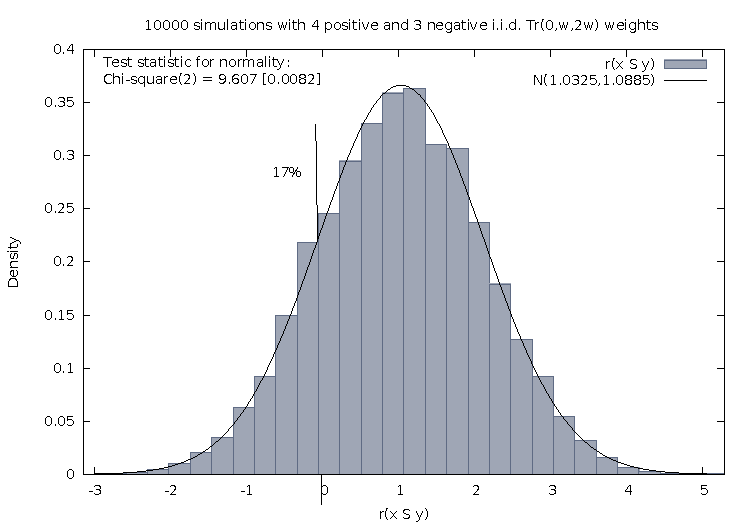
\includegraphics[width=12cm]{Figures/simulLikelihood.pdf}
\caption{Distribution of $10\,000$ random outranking characteristic values.}
\label{fig:18.3}       % Give a unique label
\end{figure}
Indeed, $\tilde{r}(x \geq y) \leadsto Y = \mathcal{N}(1.03,1.089)$, with an empirical probability of observing a negative majority margin of about $17\%$.
\end{example}

\section{Confidence level of outranking digraphs}
\label{sec:18.3}

Now, following the classical outranking approach (see \citep{BIS-2013}), we may say, from an epistemic perspective, that decision action $x$ \emph{outranks} decision action $y$ at \emph{confidence} level $\alpha \%$, when
\begin{itemize}
\item An expected majority of criteria validates, at confidence level $\alpha \%$ or higher, a global ``\emph{at least as good as}'' situation between $x$ and $y$, and
\item no considerably less performing is observed on a discordant criterion.
\end{itemize}
Dually, decision action $x$ \emph{does not outrank} decision action $y$ at
confidence level $\alpha \%$, when
\begin{itemize}
\item An expected majority of criteria at confidence level $\alpha \%$ or higher, invalidates a global ``\emph{at least as good as}'' situation between $x$ and $y$, and
\item no considerably better performing situation is observed on a discordant criterion.
\end{itemize}

\noindent \textbf{Time for a coded example}
Let us consider the following random performance tableau.
\begin{lstlisting}[basicstyle=\scriptsize]
>>> from randomPerfTabs import RandomPerformanceTableau
>>> t = RandomPerformanceTableau(\
...          numberOfActions=7,\
...          numberOfCriteria=7,seed=100)
>>> t.showPerformanceTableau(Transposed=True)
  *----  performance tableau -----*
  criteria | weights |  'a1'   'a2'   'a3'   'a4'   'a5'   'a6'   'a7'   
  ---------|----------------------------------------------------------
     'g1'  |     1   | 15.17  44.51  57.87  58.00  24.22  29.10  96.58  
     'g2'  |     1   | 82.29  43.90    NA   35.84  29.12  34.79  62.22  
     'g3'  |     1   | 44.23  19.10  27.73  41.46  22.41  21.52  56.90  
     'g4'  |     1   | 46.37  16.22  21.53  51.16  77.01  39.35  32.06  
     'g5'  |     1   | 47.67  14.81  79.70  67.48    NA   90.72  80.16  
     'g6'  |     1   | 69.62  45.49  22.03  33.83  31.83    NA   48.80  
     'g7'  |     1   | 82.88  41.66  12.82  21.92  75.74  15.45   6.05  
\end{lstlisting}

For the corresponding confident outranking digraph, we require a confidence level of $\alpha = 90\%$.

The \texttt{ConfidentBipolarOutrankingDigraph} class provides such a construction.
\begin{lstlisting}
>>> from outrankingDigraphs import\
...        ConfidentBipolarOutrankingDigraph   
>>> g90 = ConfidentBipolarOutrankingDigraph(t,confidence=90)
>>> g90
  *------- Object instance description ------*
   Instance class      : ConfidentBipolarOutrankingDigraph
   Instance name       : rel_randomperftab_CLT
   Actions           : 7
   Criteria          : 7
   Size                : 15
   Uncertainty model   : triangular(a=0,b=2w)
   Likelihood domain   : [-1.0;+1.0]
   Confidence level    : 0.80 (90.0%)
   Confident majority  : 0.14 (57.1%)
   Determinateness (%) : 62.07
   Valuation domain    : [-1.00;1.00]
   Attributes          : ['name', 'bipolarConfidenceLevel',
                 'distribution', 'betaParameter', 'actions',
                 'order', 'valuationdomain', 'criteria',
                 'evaluation', 'concordanceRelation',
                 'vetos', 'negativeVetos',
                 'largePerformanceDifferencesCount',
                 'likelihoods', 'confidenceCutLevel',
                 'relation', 'gamma', 'notGamma']
\end{lstlisting}

The resulting $90\%$-confident expected outranking relation is shown below.
\begin{lstlisting}[basicstyle=\scriptsize]
>>> g90.showRelationTable(LikelihoodDenotation=True)
  * ---- Outranking Relation Table -----
    r/(lh) |  'a1'    'a2'    'a3'    'a4'    'a5'    'a6'    'a7'	 
    -------|------------------------------------------------------
     'a1'  | +0.00   +0.71   +0.29   +0.29   +0.29   +0.29   +0.00  
           | ( - )  (+1.00) (+0.95) (+0.95) (+0.95) (+0.95) (+0.65) 
     'a2'  | -0.71   +0.00   -0.29   +0.00   +0.00   +0.29   -0.57  
           |(-1.00)  ( - )  (-0.95) (-0.65) (+0.73) (+0.95) (-1.00) 
     'a3'  | -0.29   +0.29   +0.00   -0.29   +0.00   +0.00   -0.29  
           |(-0.95) (+0.95)  ( - )  (-0.95) (-0.73) (-0.00) (-0.95) 
     'a4'  | +0.00   +0.00   +0.57   +0.00   +0.29   +0.57   -0.43  
       	   |(-0.00) (+0.65) (+1.00)  ( - )  (+0.95) (+1.00) (-0.99) 
     'a5'  | -0.29   +0.00   +0.00   +0.00   +0.00   +0.29   -0.29  
           |(-0.95) (-0.00) (+0.73) (-0.00)  ( - )  (+0.99) (-0.95) 
     'a6'  | -0.29   +0.00   +0.00   -0.29   +0.00   +0.00   +0.00  
           |(-0.95) (-0.00) (+0.73) (-0.95) (+0.73)  ( - )  (-0.00) 
     'a7'  | +0.00   +0.71   +0.57   +0.43   +0.29   +0.00   +0.00  
           |(-0.65) (+1.00) (+1.00) (+0.99) (+0.95) (-0.00)  ( - )  
    Valuation domain   : [-1.000; +1.000] 
    Uncertainty model  : triangular(a=2.0,b=2.0) 
    Likelihood domain  : [-1.0;+1.0] 
    Confidence level   : 0.80 (90.0%) 
    Confident majority : 0.14 (57.1%) 
    Determinateness    : 0.24 (62.1%)
\end{lstlisting}

The ($lh$) figures, indicated in the table above, correspond to bipolar likelihoods and the required bipolar confidence level equals $(0.90+1.0)/2 = 0.80$ (see Line 22 above). Action 'a1' thus confidently outranks all other actions, except 'a7' where the actual likelihood ($+0.65$) is lower than the required one ($0.80$) and we furthermore observe a considerable counter-performance on criterion 'g1'.

Notice also the lack of confidence in the outranking situations we observe between action 'a2' and actions 'a4' and 'a5'. In the deterministic case we would have $r(a2 \geq a4) \,=\, -0.143$ and $r(a2 \geq a5) \,=\, +0.143$ . All outranking situations with a characteristic value lower or equal to $abs(0.143)$, i.e. a majority support of $1.143/2 = 57.1\%$ and less, appear indeed to be \emph{not confident} at $\alpha$ level $90\%$ (see Line 23 above).

We may draw the corresponding strict $90\%$-confident outranking digraph, oriented by its initial and terminal strict prekernels (see Fig. \ref{fig:18.4}).
\begin{lstlisting}
>>> gcd90 = ~ (-g90)
>>> gcd90.showPreKernels()
  *--- Computing preKernels ---*
   Dominant preKernels :
    ['a1', 'a7']
       independence :  0.0
       dominance    :  0.2857
       absorbency   :  -0.7143
       covering     :  0.800
   Absorbent preKernels :
    ['a2', 'a5', 'a6']
       independence :  0.0
       dominance    :  -0.2857
       absorbency   :  0.2857
       covered      :  0.583
>>> gcd90.exportGraphViz(fileName='confidentOutranking',
...        bestChoice=['a1', 'a7'],worstChoice=['a2', 'a5', 'a6'])
  *---- exporting a dot file for GraphViz tools ---------*
   Exporting to confidentOutranking.dot
   dot -Grankdir=BT -Tpng confidentOutranking.dot\
                    -o confidentOutranking.png
\end{lstlisting}

\begin{figure}[h]
\sidecaption
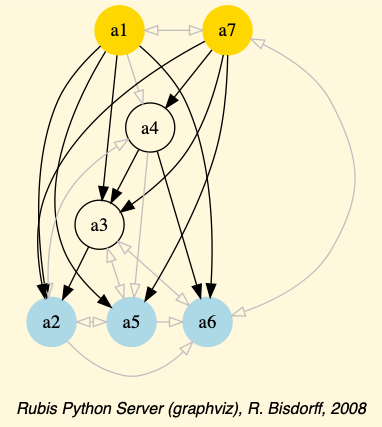
\includegraphics[width=6cm]{Figures/confidentOutranking.png}
\caption{90\%-confident strict outranking digraph oriented by its prekernels}
\label{fig:18.4}       % Give a unique label
\end{figure}

Now, what becomes this 90\%-confident outranking digraph when we require a stronger confidence level of, say $99\%$?
\begin{lstlisting}[basicstyle=\scriptsize]
>>> g99 = ConfidentBipolarOutrankingDigraph(t,confidence=99)
>>> g99.showRelationTable()
  * ---- Outranking Relation Table -----
   r/(lh) |  'a1'    'a2'    'a3'    'a4'    'a5'    'a6'    'a7'	 
   -------|------------------------------------------------------
    'a1'  |  +0.00   +0.71   +0.00   +0.00   +0.00   +0.00   +0.00  
          |  ( - )  (+1.00) (+0.95) (+0.95) (+0.95) (+0.95) (+0.65) 
    'a2'  |  -0.71   +0.00   +0.00   +0.00   +0.00   +0.00   -0.57  
          | (-1.00)  ( - )  (-0.95) (-0.65) (+0.73) (+0.95) (-1.00) 
    'a3'  |  +0.00   +0.00   +0.00   +0.00   +0.00   +0.00   +0.00  
          | (-0.95) (+0.95)  ( - )  (-0.95) (-0.73) (-0.00) (-0.95) 
    'a4'  |  +0.00   +0.00   +0.57   +0.00   +0.00   +0.57   -0.43  
          | (-0.00) (+0.65) (+1.00)  ( - )  (+0.95) (+1.00) (-0.99) 
    'a5'  |  +0.00   +0.00   +0.00   +0.00   +0.00   +0.29   +0.00  
          | (-0.95) (-0.00) (+0.73) (-0.00)  ( - )  (+0.99) (-0.95) 
    'a6'  |  +0.00   +0.00   +0.00   +0.00   +0.00   +0.00   +0.00  
          | (-0.95) (-0.00) (+0.73) (-0.95) (+0.73)  ( - )  (-0.00) 
    'a7'  |  +0.00   +0.71   +0.57   +0.43   +0.00   +0.00   +0.00  
          | (-0.65) (+1.00) (+1.00) (+0.99) (+0.95) (-0.00)  ( - )  
    Valuation domain   : [-1.000; +1.000] 
    Uncertainty model  : triangular(a=2.0,b=2.0) 
    Likelihood domain  : [-1.0;+1.0] 
    Confidence level   : 0.98 (99.0%) 
    Confident majority : 0.29 (64.3%) 
    Determinateness    : 0.13 (56.6%)
\end{lstlisting}

At $99\%$ confidence, the minimal required significance majority support amounts to $64.3\%$ (see Line 24 above). As a result, most outranking situations don't get anymore validated, like the outranking situations between action 'a1' and actions 'a3', 'a4', 'a5' and 'a6' (see Line 5 above). The overall epistemic determination of the digraph consequently drops from $.1\%$ to $56.6\%$ (see Line 25).

Finally, what becomes the previous $90\%$-confident outranking digraph if the uncertainty concerning the criteria significance weights is modelled with a larger variance, like \emph{uniform} variates (see Line 2 below).
\begin{lstlisting}[basicstyle=\scriptsize]
>>> gu90 = ConfidentBipolarOutrankingDigraph(t,\
...           confidence=90,distribution='uniform')
>>> gu90.showRelationTable()
  * ---- Outranking Relation Table -----
  r/(lh) |   'a1'    'a2'    'a3'    'a4'    'a5'    'a6'    'a7'	 
  -------|-------------------------------------------------------
    'a1' |  +0.00   +0.71   +0.29   +0.29   +0.29   +0.29   +0.00  
         |  ( - )  (+1.00) (+0.84) (+0.84) (+0.84) (+0.84) (+0.49) 
    'a2' |  -0.71   +0.00   -0.29   +0.00   +0.00   +0.29   -0.57  
         | (-1.00)  ( - )  (-0.84) (-0.49) (+0.56) (+0.84) (-1.00) 
    'a3' |  -0.29   +0.29   +0.00   -0.29   +0.00   +0.00   -0.29  
         | (-0.84) (+0.84)  ( - )  (-0.84) (-0.56) (-0.00) (-0.84) 
    'a4' |  +0.00   +0.00   +0.57   +0.00   +0.29   +0.57   -0.43  
         | (-0.00) (+0.49) (+1.00)  ( - )  (+0.84) (+1.00) (-0.95) 
    'a5' |  -0.29   +0.00   +0.00   +0.00   +0.00   +0.29   -0.29  
         | (-0.84) (-0.00) (+0.56) (-0.00)  ( - )  (+0.92) (-0.84) 
    'a6' |  -0.29   +0.00   +0.00   -0.29   +0.00   +0.00   +0.00  
         | (-0.84) (-0.00) (+0.56) (-0.84) (+0.56)  ( - )  (-0.00) 
    'a7' |  +0.00   +0.71   +0.57   +0.43   +0.29   +0.00   +0.00  
         | (-0.49) (+1.00) (+1.00) (+0.95) (+0.84) (-0.00)  ( - )  
    Valuation domain   : [-1.000; +1.000] 
    Uncertainty model  : uniform(a=2.0,b=2.0) 
    Likelihood domain  : [-1.0;+1.0] 
    Confidence level   : 0.80 (90.0%) 
    Confident majority : 0.14 (57.1%) 
    Determinateness    : 0.24 (62.1%)
\end{lstlisting}

Despite lower likelihood values (see the $g90$ relation table above), we keep the same confident majority level of $57.1\%$ (see Line 25 above) and, hence, also the same $90\%$-confident outranking digraph.

For concluding, it is worthwhile noticing again that it is in fact the \emph{neutral} value of our bipolar-valued epistemic logic that allows us to easily handle $\alpha\%$ confidence or not of outranking situations when confronted with uncertain criteria significances. Remarkable furthermore is the usage, the standard Gaussian error function (erf) provides by delivering \emph{signed} likelihood values immediately concerning either a positive relational statement, or when negative, its negated version. 
 
%%%%%%% The chapter bibliography
%\normallatexbib
\clearpage
%\phantomsection
%\addcontentsline{toc}{section}{Chapter Bibliography}
\bibliographystyle{spbasic}
%\typeout{}
\bibliography{03-backMatters/reference}
%\chapter[On confident outrankings]{On confident outrankings with uncertain criteria significance weights}
\label{sec:18}

\abstract*{When modelling preferences following the outranking approach, the signs of the majority margins do sharply distribute validation and invalidation of pairwise outranking situations. How can we be confident in the resulting outranking digraph, when we acknowledge the usual imprecise knowledge of criteria significance weights coupled with small majority margins? To answer this question, one usually requires \emph{qualified} majority margins for confirming outranking situations. But how to choose such a qualifying majority level: two third, three fourth of the significances ? In this chapter we propose to link the qualifying significance majority with a required $\alpha\%$-confidence level. We model therefore the significance weights as random variables following more or less widespread distributions around an average significance value that corresponds to the given deterministic weight. As the bipolar-valued random credibility of an outranking statement hence results from the simple sum of positive or negative independent random variables, we may apply the Central Limit Theorem (CLT) for computing the bipolar likelihood that the expected majority margin will indeed be positive, respectively negative.}

\abstract{When modelling preferences following the outranking approach, the signs of the majority margins do sharply distribute validation and invalidation of pairwise outranking situations. How can we be confident in the resulting outranking digraph, when we acknowledge the usual imprecise knowledge of criteria significance weights coupled with small majority margins? To answer this question, one usually requires \emph{qualified} majority margins for confirming outranking situations. But how to choose such a qualifying majority level: two third, three fourth of the significances ? In this chapter we propose to link the qualifying significance majority with a required $\alpha\%$-confidence level. We model therefore the significance weights as random variables following more or less widespread distributions around an average significance value that corresponds to the given deterministic weight. As the bipolar-valued random credibility of an outranking statement hence results from the simple sum of positive or negative independent random variables, we may apply the Central Limit Theorem (CLT) for computing the bipolar likelihood that the expected majority margin will indeed be positive, respectively negative.}

\section{Modelling uncertain criteria significances}
\label{sec:18.1}

Let us consider the significance weights of a family $F$ of $m$ criteria to be independent random variables $W_j$, distributing the potential significance weights of each criterion $j = 1, ..., m$ around a mean value $E(W_j)$ with variance $V(W_j)$.

Choosing a specific stochastic model of uncertainty is usually application specific. In the limited scope of this chapter, we will illustrate the consequence of this design decision on the resulting outranking modelling with four slightly different models for taking into account the uncertainty with which we know the numerical significance weights: \emph{uniform}, \emph{triangular}, and two models of \emph{Beta laws}, one more widespread and, the other, more concentrated.

When considering, for instance, that the potential range of a significance weight is distributed between $0$ and two times its mean value, we obtain the following random variates:
\begin{itemize}
\item A continuous \emph{uniform} distribution on the range $0$ to $2E(W_j)$. Thus $W_j \leadsto U(0, 2E(W_j))$ and $V(W_j) = 1/3(E(W_j))^2$;
\item A \emph{symmetric beta} distribution with, for instance, parameters  $\alpha = 2$ and $\beta = 2$. Thus, $W_i \leadsto Beta(2,2) \times 2E(W_j)$ and $V(W_j) = 1/5(E(Wj))^2$;
\item A \emph{symmetric triangular} distribution on the same range wit mode $E(W_j)$. Thus $W_j \leadsto Tr(0, 2E(W_j), E(Wj))$ with $V(W_j) = 1/6(E(Wj))^2$;
\item A \emph{narrower beta} distribution with, for instance, parameters $\alpha = 4$ and $\beta = 4$. Thus $W_j \leadsto Beta(4,4) \times 2E(W_j)$ , $V(W_j) = 1/9(E(W_j))^2$.
\end{itemize}
\begin{figure}[h]
%\sidecaption
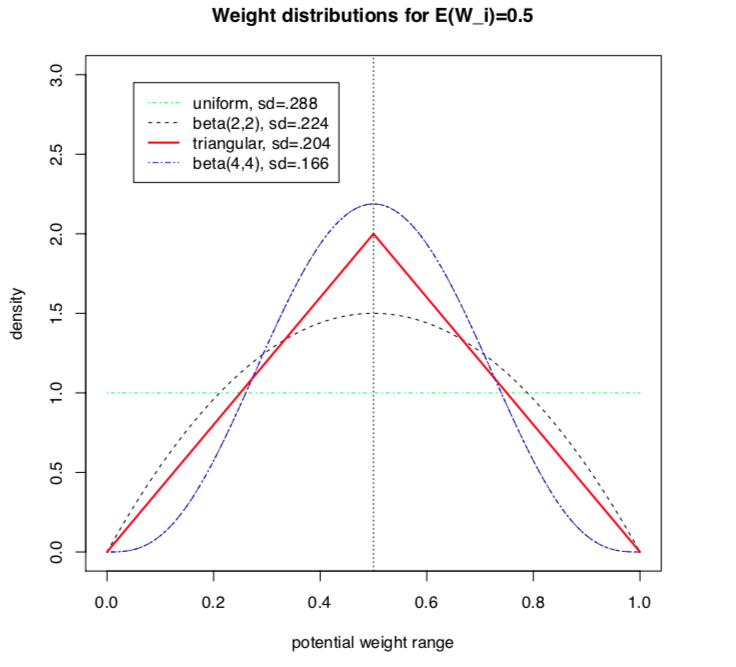
\includegraphics[width=12cm]{Figures/weightDistributions.png}
\caption{Four models of uncertain significance weights}
\label{fig:18.1}       % Give a unique label
\end{figure}
It is worthwhile noticing that these four uncertainty models all admit the same expected value, $E(W_j)$, however, with a respective variance which goes decreasing from $1/3$, to $1/9$ of the square of $E(W_j)$ (see Fig. \ref{fig:18.1}).

\section{Bipolar-valued likelihood of outranking situations}
\label{sec:18.2}

Let $A = \{x, y, z,...\}$ be a finite set of $n$ potential decision actions, evaluated on $F = \{1,..., m\}$ --a finite and coherent family of $m$ performance criteria. On each criterion $j \in F$, the decision actions are evaluated on a real performance scale $[0; M_j ]$, supporting an upper-closed indifference threshold $indj$ and a lower-closed preference threshold $prj$ such that $0 \leq indj < prj \leq M_j$. The marginal performance of object $x$ on criterion $j$ is denoted $x_j$. Each criterion $j$ is thus characterising a marginal double threshold order $\geq_j$ on $A$:
\begin{equation}
  r(x \geq_j y) \; = \; \begin{cases} +1 \quad \text{if} \quad x_j - y_j \leq -ind_j,\\  -1 \quad \text{if} \quad x_j - y_j \leq -pr_j,\\ 0 \quad \text{otherwise}. \end{cases}
\end{equation}

Semantics of the marginal bipolar-valued characteristic function:
\begin{itemize}
\item $+1$ signifies $x$ is performing at least as good as $y$ on criterion $j$,
\item $-1$ signifies that $x$ is not performing at least as good as $y$ on criterion $j$,
\item $0$ signifies that it is unclear whether, on criterion $j$, $x$ is performing at least as good as $y$.
\end{itemize}
\begin{figure}[h]
%\sidecaption
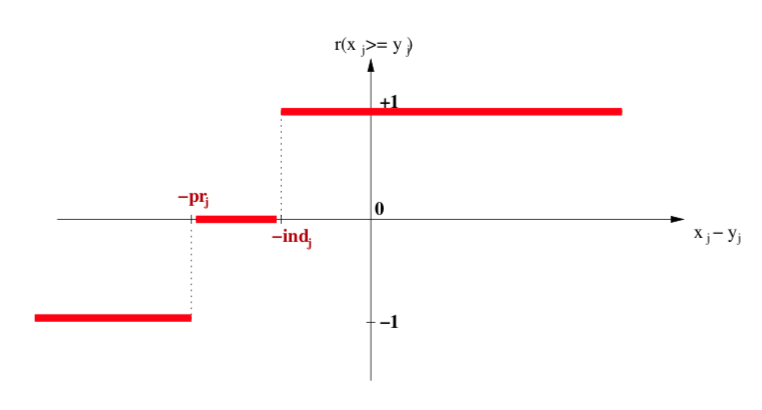
\includegraphics[width=11cm]{Figures/rCharacteristic.png}
\caption{Bipolar-valued outranking characteristic function.}
\label{fig:18.2}       % Give a unique label
\end{figure}
Each criterion $j$ in $F$ contributes the random significance $W_j$ of his ``\emph{at least as good as}'' characteristic $r(x \geq_j y)$ to the global characteristic $\tilde{r}(x \geq y)$ in the following way:
\begin{equation}
      \tilde{r}(x \geq y) \; = \; \sum_{j \in F} W_j \times r(x \geq_j y) )
    \end{equation}
Thus, $\tilde{r}(x \geq y)$ becomes a simple sum of positive or negative independent random variables with known means and variances where $\tilde{r}(x \geq y) \, > \, 0$ signifies $x$ is globally performing at least as good as $y$, $\tilde{r}(x \geq y) \, < \, 0$ signifies that $x$ is not globally performing at least as good as $y$, and $\tilde{r}(x \geq y)\,=\,0$ signifies that it is unclear whether $x$ is globally performing at least as good as $y$.

From the \emph{Central Limit Theorem} (CLT), we know that such a sum of random variables leads, with $m$ getting large, to a Gaussian distribution $Y$ with
\begin{eqnarray}
E(Y ) = &\sum_{j \in F} \big(\,E(W_j) \times r(x \geq_j y)\,\big), \text{and}\\
V(Y) = &\sum_{j \in F} \big(\,V(W_j)\times |r(x \geq_j y)|\,\big).
\end{eqnarray}
And the \emph{likelihood of validation}, respectively \emph{invalidation} of an ``\emph{at least as good as}'' situation, denoted $lh(x \geq y)$,  may hence be assessed by the probability $P(Y > 0) = 1.0 - P(Y \leq 0)$ that $Y$ takes a positive, resp. $P(Y < 0)$ takes a negative value. In the bipolar-valued case here, we can judiciously make usage of the standard Gaussian \emph{error function} , i.e. the bipolar $2P(Z) - 1.0$ version of the standard Gaussian $P(Z)$ probability distribution function:
\begin{equation}
  lh(x \geq y) \;=\; -\text{erf}\big(\frac{1}{\sqrt{2}}\frac{-E(Y)}{\sqrt{V(Y)}} \big)
\end{equation}
The range of the bipolar-valued $lh(x \geq y)$ hence becomes $[-1.0;+1.0]$, and $-lh(x \geq y) \,=\, lh(x \not\geq y)$ , i.e. a \emph{negative likelihood} represents the likelihood of the correspondent \emph{negated} ``\emph{at least as good as}'' situation. A likelihood of $+1.0$ (resp. $-1.0$) means the corresponding preferential situation appears \emph{certainly} validated (resp. invalidated).

\begin{example} Let $x$ and $y$ be evaluated wrt 7 equisignificant criteria; Four criteria positively support that $x$ is \emph{as least as good performing} than $y$ and three criteria support that $x$ is \emph{not at least as good} performing than $y$. Suppose $E(W_j) = w$ for $j = 1,...,7$ and $W_j \leadsto Tr(0, 2w, w)$ for $j = 1,...7$. The expected value of the global ``\emph{at least as good as}'' characteristic value becomes: $E\big(\tilde{r}(x \geq y)\big)\, = \, 4w - 3w = w$ with a variance $V\big(\tilde{r}(x \geq y)\big)\,=\, 7\frac{1}{6}w^2$. 

If $w = 1$, $E\big(\tilde{r}(x \geq y)\big)\, = \, 1$ and $sd\big(\tilde{r}(x \geq y)\big)\,=\, 1.08$. By the CLT, the bipolar likelihood of the \emph{at least as good} performing situation becomes: $lh(x \geq y)\,=\, 0.66$, which corresponds to a global support of $(0.66 + 1.0)/2 = 83\%$ of the criteria significance weights.

A \emph{Monte Carlo} simulation with $10\,000$ runs empirically confirms the effective convergence to a Gaussian (see Fig. \ref{fig:18.3} realised with \emph{gretl} \footnote{The Gnu Regression, Econometrics and Time-series Library http://gretl.sourceforge.net/ .}.
\begin{figure}[h]
%\sidecaption
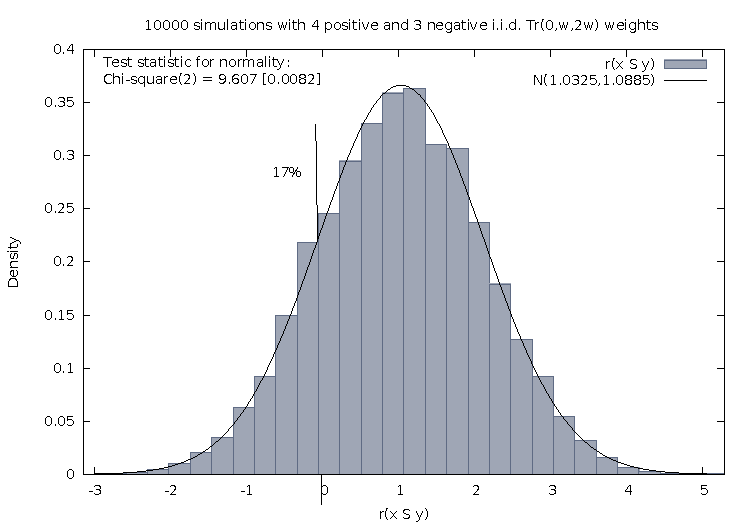
\includegraphics[width=12cm]{Figures/simulLikelihood.pdf}
\caption{Distribution of $10\,000$ random outranking characteristic values.}
\label{fig:18.3}       % Give a unique label
\end{figure}
Indeed, $\tilde{r}(x \geq y) \leadsto Y = \mathcal{N}(1.03,1.089)$, with an empirical probability of observing a negative majority margin of about $17\%$.
\end{example}

\section{Confidence level of outranking digraphs}
\label{sec:18.3}

Now, following the classical outranking approach (see \citep{BIS-2013}), we may say, from an epistemic perspective, that decision action $x$ \emph{outranks} decision action $y$ at \emph{confidence} level $\alpha \%$, when
\begin{itemize}
\item An expected majority of criteria validates, at confidence level $\alpha \%$ or higher, a global ``\emph{at least as good as}'' situation between $x$ and $y$, and
\item no considerably less performing is observed on a discordant criterion.
\end{itemize}
Dually, decision action $x$ \emph{does not outrank} decision action $y$ at
confidence level $\alpha \%$, when
\begin{itemize}
\item An expected majority of criteria at confidence level $\alpha \%$ or higher, invalidates a global ``\emph{at least as good as}'' situation between $x$ and $y$, and
\item no considerably better performing situation is observed on a discordant criterion.
\end{itemize}

\noindent \textbf{Time for a coded example}
Let us consider the following random performance tableau.
\begin{lstlisting}[basicstyle=\scriptsize]
>>> from randomPerfTabs import RandomPerformanceTableau
>>> t = RandomPerformanceTableau(\
...          numberOfActions=7,\
...          numberOfCriteria=7,seed=100)
>>> t.showPerformanceTableau(Transposed=True)
  *----  performance tableau -----*
  criteria | weights |  'a1'   'a2'   'a3'   'a4'   'a5'   'a6'   'a7'   
  ---------|----------------------------------------------------------
     'g1'  |     1   | 15.17  44.51  57.87  58.00  24.22  29.10  96.58  
     'g2'  |     1   | 82.29  43.90    NA   35.84  29.12  34.79  62.22  
     'g3'  |     1   | 44.23  19.10  27.73  41.46  22.41  21.52  56.90  
     'g4'  |     1   | 46.37  16.22  21.53  51.16  77.01  39.35  32.06  
     'g5'  |     1   | 47.67  14.81  79.70  67.48    NA   90.72  80.16  
     'g6'  |     1   | 69.62  45.49  22.03  33.83  31.83    NA   48.80  
     'g7'  |     1   | 82.88  41.66  12.82  21.92  75.74  15.45   6.05  
\end{lstlisting}

For the corresponding confident outranking digraph, we require a confidence level of $\alpha = 90\%$.

The \texttt{ConfidentBipolarOutrankingDigraph} class provides such a construction.
\begin{lstlisting}
>>> from outrankingDigraphs import\
...        ConfidentBipolarOutrankingDigraph   
>>> g90 = ConfidentBipolarOutrankingDigraph(t,confidence=90)
>>> g90
  *------- Object instance description ------*
   Instance class      : ConfidentBipolarOutrankingDigraph
   Instance name       : rel_randomperftab_CLT
   Actions           : 7
   Criteria          : 7
   Size                : 15
   Uncertainty model   : triangular(a=0,b=2w)
   Likelihood domain   : [-1.0;+1.0]
   Confidence level    : 0.80 (90.0%)
   Confident majority  : 0.14 (57.1%)
   Determinateness (%) : 62.07
   Valuation domain    : [-1.00;1.00]
   Attributes          : ['name', 'bipolarConfidenceLevel',
                 'distribution', 'betaParameter', 'actions',
                 'order', 'valuationdomain', 'criteria',
                 'evaluation', 'concordanceRelation',
                 'vetos', 'negativeVetos',
                 'largePerformanceDifferencesCount',
                 'likelihoods', 'confidenceCutLevel',
                 'relation', 'gamma', 'notGamma']
\end{lstlisting}

The resulting $90\%$-confident expected outranking relation is shown below.
\begin{lstlisting}[basicstyle=\scriptsize]
>>> g90.showRelationTable(LikelihoodDenotation=True)
  * ---- Outranking Relation Table -----
    r/(lh) |  'a1'    'a2'    'a3'    'a4'    'a5'    'a6'    'a7'	 
    -------|------------------------------------------------------
     'a1'  | +0.00   +0.71   +0.29   +0.29   +0.29   +0.29   +0.00  
           | ( - )  (+1.00) (+0.95) (+0.95) (+0.95) (+0.95) (+0.65) 
     'a2'  | -0.71   +0.00   -0.29   +0.00   +0.00   +0.29   -0.57  
           |(-1.00)  ( - )  (-0.95) (-0.65) (+0.73) (+0.95) (-1.00) 
     'a3'  | -0.29   +0.29   +0.00   -0.29   +0.00   +0.00   -0.29  
           |(-0.95) (+0.95)  ( - )  (-0.95) (-0.73) (-0.00) (-0.95) 
     'a4'  | +0.00   +0.00   +0.57   +0.00   +0.29   +0.57   -0.43  
       	   |(-0.00) (+0.65) (+1.00)  ( - )  (+0.95) (+1.00) (-0.99) 
     'a5'  | -0.29   +0.00   +0.00   +0.00   +0.00   +0.29   -0.29  
           |(-0.95) (-0.00) (+0.73) (-0.00)  ( - )  (+0.99) (-0.95) 
     'a6'  | -0.29   +0.00   +0.00   -0.29   +0.00   +0.00   +0.00  
           |(-0.95) (-0.00) (+0.73) (-0.95) (+0.73)  ( - )  (-0.00) 
     'a7'  | +0.00   +0.71   +0.57   +0.43   +0.29   +0.00   +0.00  
           |(-0.65) (+1.00) (+1.00) (+0.99) (+0.95) (-0.00)  ( - )  
    Valuation domain   : [-1.000; +1.000] 
    Uncertainty model  : triangular(a=2.0,b=2.0) 
    Likelihood domain  : [-1.0;+1.0] 
    Confidence level   : 0.80 (90.0%) 
    Confident majority : 0.14 (57.1%) 
    Determinateness    : 0.24 (62.1%)
\end{lstlisting}

The ($lh$) figures, indicated in the table above, correspond to bipolar likelihoods and the required bipolar confidence level equals $(0.90+1.0)/2 = 0.80$ (see Line 22 above). Action 'a1' thus confidently outranks all other actions, except 'a7' where the actual likelihood ($+0.65$) is lower than the required one ($0.80$) and we furthermore observe a considerable counter-performance on criterion 'g1'.

Notice also the lack of confidence in the outranking situations we observe between action 'a2' and actions 'a4' and 'a5'. In the deterministic case we would have $r(a2 \geq a4) \,=\, -0.143$ and $r(a2 \geq a5) \,=\, +0.143$ . All outranking situations with a characteristic value lower or equal to $abs(0.143)$, i.e. a majority support of $1.143/2 = 57.1\%$ and less, appear indeed to be \emph{not confident} at $\alpha$ level $90\%$ (see Line 23 above).

We may draw the corresponding strict $90\%$-confident outranking digraph, oriented by its initial and terminal strict prekernels (see Fig. \ref{fig:18.4}).
\begin{lstlisting}
>>> gcd90 = ~ (-g90)
>>> gcd90.showPreKernels()
  *--- Computing preKernels ---*
   Dominant preKernels :
    ['a1', 'a7']
       independence :  0.0
       dominance    :  0.2857
       absorbency   :  -0.7143
       covering     :  0.800
   Absorbent preKernels :
    ['a2', 'a5', 'a6']
       independence :  0.0
       dominance    :  -0.2857
       absorbency   :  0.2857
       covered      :  0.583
>>> gcd90.exportGraphViz(fileName='confidentOutranking',
...        bestChoice=['a1', 'a7'],worstChoice=['a2', 'a5', 'a6'])
  *---- exporting a dot file for GraphViz tools ---------*
   Exporting to confidentOutranking.dot
   dot -Grankdir=BT -Tpng confidentOutranking.dot\
                    -o confidentOutranking.png
\end{lstlisting}

\begin{figure}[h]
\sidecaption
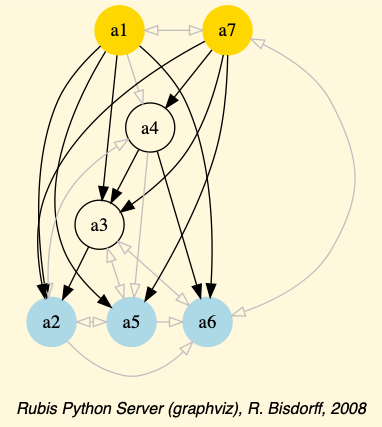
\includegraphics[width=6cm]{Figures/confidentOutranking.png}
\caption{90\%-confident strict outranking digraph oriented by its prekernels}
\label{fig:18.4}       % Give a unique label
\end{figure}

Now, what becomes this 90\%-confident outranking digraph when we require a stronger confidence level of, say $99\%$?
\begin{lstlisting}[basicstyle=\scriptsize]
>>> g99 = ConfidentBipolarOutrankingDigraph(t,confidence=99)
>>> g99.showRelationTable()
  * ---- Outranking Relation Table -----
   r/(lh) |  'a1'    'a2'    'a3'    'a4'    'a5'    'a6'    'a7'	 
   -------|------------------------------------------------------
    'a1'  |  +0.00   +0.71   +0.00   +0.00   +0.00   +0.00   +0.00  
          |  ( - )  (+1.00) (+0.95) (+0.95) (+0.95) (+0.95) (+0.65) 
    'a2'  |  -0.71   +0.00   +0.00   +0.00   +0.00   +0.00   -0.57  
          | (-1.00)  ( - )  (-0.95) (-0.65) (+0.73) (+0.95) (-1.00) 
    'a3'  |  +0.00   +0.00   +0.00   +0.00   +0.00   +0.00   +0.00  
          | (-0.95) (+0.95)  ( - )  (-0.95) (-0.73) (-0.00) (-0.95) 
    'a4'  |  +0.00   +0.00   +0.57   +0.00   +0.00   +0.57   -0.43  
          | (-0.00) (+0.65) (+1.00)  ( - )  (+0.95) (+1.00) (-0.99) 
    'a5'  |  +0.00   +0.00   +0.00   +0.00   +0.00   +0.29   +0.00  
          | (-0.95) (-0.00) (+0.73) (-0.00)  ( - )  (+0.99) (-0.95) 
    'a6'  |  +0.00   +0.00   +0.00   +0.00   +0.00   +0.00   +0.00  
          | (-0.95) (-0.00) (+0.73) (-0.95) (+0.73)  ( - )  (-0.00) 
    'a7'  |  +0.00   +0.71   +0.57   +0.43   +0.00   +0.00   +0.00  
          | (-0.65) (+1.00) (+1.00) (+0.99) (+0.95) (-0.00)  ( - )  
    Valuation domain   : [-1.000; +1.000] 
    Uncertainty model  : triangular(a=2.0,b=2.0) 
    Likelihood domain  : [-1.0;+1.0] 
    Confidence level   : 0.98 (99.0%) 
    Confident majority : 0.29 (64.3%) 
    Determinateness    : 0.13 (56.6%)
\end{lstlisting}

At $99\%$ confidence, the minimal required significance majority support amounts to $64.3\%$ (see Line 24 above). As a result, most outranking situations don't get anymore validated, like the outranking situations between action 'a1' and actions 'a3', 'a4', 'a5' and 'a6' (see Line 5 above). The overall epistemic determination of the digraph consequently drops from $.1\%$ to $56.6\%$ (see Line 25).

Finally, what becomes the previous $90\%$-confident outranking digraph if the uncertainty concerning the criteria significance weights is modelled with a larger variance, like \emph{uniform} variates (see Line 2 below).
\begin{lstlisting}[basicstyle=\scriptsize]
>>> gu90 = ConfidentBipolarOutrankingDigraph(t,\
...           confidence=90,distribution='uniform')
>>> gu90.showRelationTable()
  * ---- Outranking Relation Table -----
  r/(lh) |   'a1'    'a2'    'a3'    'a4'    'a5'    'a6'    'a7'	 
  -------|-------------------------------------------------------
    'a1' |  +0.00   +0.71   +0.29   +0.29   +0.29   +0.29   +0.00  
         |  ( - )  (+1.00) (+0.84) (+0.84) (+0.84) (+0.84) (+0.49) 
    'a2' |  -0.71   +0.00   -0.29   +0.00   +0.00   +0.29   -0.57  
         | (-1.00)  ( - )  (-0.84) (-0.49) (+0.56) (+0.84) (-1.00) 
    'a3' |  -0.29   +0.29   +0.00   -0.29   +0.00   +0.00   -0.29  
         | (-0.84) (+0.84)  ( - )  (-0.84) (-0.56) (-0.00) (-0.84) 
    'a4' |  +0.00   +0.00   +0.57   +0.00   +0.29   +0.57   -0.43  
         | (-0.00) (+0.49) (+1.00)  ( - )  (+0.84) (+1.00) (-0.95) 
    'a5' |  -0.29   +0.00   +0.00   +0.00   +0.00   +0.29   -0.29  
         | (-0.84) (-0.00) (+0.56) (-0.00)  ( - )  (+0.92) (-0.84) 
    'a6' |  -0.29   +0.00   +0.00   -0.29   +0.00   +0.00   +0.00  
         | (-0.84) (-0.00) (+0.56) (-0.84) (+0.56)  ( - )  (-0.00) 
    'a7' |  +0.00   +0.71   +0.57   +0.43   +0.29   +0.00   +0.00  
         | (-0.49) (+1.00) (+1.00) (+0.95) (+0.84) (-0.00)  ( - )  
    Valuation domain   : [-1.000; +1.000] 
    Uncertainty model  : uniform(a=2.0,b=2.0) 
    Likelihood domain  : [-1.0;+1.0] 
    Confidence level   : 0.80 (90.0%) 
    Confident majority : 0.14 (57.1%) 
    Determinateness    : 0.24 (62.1%)
\end{lstlisting}

Despite lower likelihood values (see the $g90$ relation table above), we keep the same confident majority level of $57.1\%$ (see Line 25 above) and, hence, also the same $90\%$-confident outranking digraph.

For concluding, it is worthwhile noticing again that it is in fact the \emph{neutral} value of our bipolar-valued epistemic logic that allows us to easily handle $\alpha\%$ confidence or not of outranking situations when confronted with uncertain criteria significances. Remarkable furthermore is the usage, the standard Gaussian error function (erf) provides by delivering \emph{signed} likelihood values immediately concerning either a positive relational statement, or when negative, its negated version. 
 
%%%%%%% The chapter bibliography
%\normallatexbib
\clearpage
%\phantomsection
%\addcontentsline{toc}{section}{Chapter Bibliography}
\bibliographystyle{spbasic}
%\typeout{}
\bibliography{03-backMatters/reference}
%\input{02-mainMatters/18-chapterConfidentOutrankings.bbl}
\bibliographystyle{spbasic}
\bibliography{03-backMatters/reference}
